\chapter{Full Posit Processing Unit (PPU)}\label{chap:posit_fullppu}

\lettrine{I}{n} this chapter, we extend the architecture seen in Section 6.5, adding the capability for arithmetic operations between posits - that is, addition, subtraction, multiplication and division.



\section{Single-stage Architecture}

Firstly, in the following sections, we will refer to a PPU design with a single stage of computation. This means that the unit is a single combinatory logic component from input to output.

Theoretically, this means that:
\begin{itemize}
    \item We are sure that, in 1 clock cycle, the component will output its result
    \item The end-to-end latency can negatively affect the drive clock fed to the unit. Indeed, if we imagine the unit being integrated into a more complex system (e.g. a full processor), its inputs and outputs will be fed from/into registers. In order to respect the timing constraints of registers, the clock period must be adjusted to the latency of the processor components. If the PPU unit is has a sufficiently large end-to-end latency, this can impact the clock frequency for the whole processor, slowing down the whole system.
\end{itemize}

From a high-level perspective, the main building blocks are highlighted in Figure \ref{fig:overview_ppu}.
The operands are converted into the general FIR datatype through the \textit{extraction} stage; the \textit{computation} stage contains addition, subtraction, multiplication, and division according to the control signal for the operation; finally, the \textit{normalization} stage contains the conversion from the computation FIR output to a posit bit-string.

\begin{figure}
    \begin{center}
    \includegraphics[width=0.9\textwidth]{figures/top.pdf}
    \caption{Single stage configuration for a PPU unit}
    \label{fig:overview_ppu}
    \end{center}
\end{figure}

\section{Datapath}

\subsection{Extraction}\label{sec:posit_extraction}

The extraction module (Figure \ref{fig:extraction_ppu}) performs a preliminary input conditioning (Figure \ref{fig:input_conditioning_module}) on the posit inputs, then it is followed by the field extraction.

The input conditioning module:
\begin{enumerate}
    \item performs operand swapping if the second operand encodes a negative value, or the second operand encodes a larger (in absolute) value than the first 
    \item detects special and trivial cases, depending on the operation considered (e.g. we have a sum and one of the two inputs is zero).
\end{enumerate} 

In the second case, the \texttt{special} signal is forwarded straight to the output of the PPU result. 

Both of the aforementioned cases can be resolved at the posit bit-string level (i.e. without the need for decoding) and don't involve the remaining two intermediate stages.

\begin{figure}
    \centering
    \includegraphics[width=0.87\textwidth]{figures/extraction.drawio.pdf}
    \caption{Extraction module}
    \label{fig:extraction_ppu}
\end{figure}

\begin{figure}
    \centering
    \includegraphics[width=0.9\textwidth]{figures/posit2fir.drawio.pdf}
    \caption{Posit to FIR module}
    \label{fig:posit2fir_ppu}
\end{figure}






\begin{figure}
    \centering
    \includegraphics[width=.75\textwidth]{figures/input_conditioning.pdf}
    \caption{Input conditioning module}
    \label{fig:input_conditioning_module}
\end{figure}



\textit{Posit to FIR} (Figure \ref{fig:posit2fir_ppu}) takes a \texttt{N}-bit bitstring encoding a posit and outputs a \texttt{FIR\_SIZE}-bit\footnote{\texttt{1 + TE\_SIZE + FRAC\_SIZE} = \texttt{1 + [(ES + 1) + (clog2(N) + 1)] + (N - 2)}} bistring encoding the concatenation of \textit{sign}, the total exponent \textit{te}, and the fraction \textit{frac}.
The most complex part of the operation is done by the \textit{posit unpack} module which extracts and decodes the posit fields. The procedure is similar to the extraction of binary32 fields; however, the implementation has more complex steps, since the size of the regime is not pre-determined.
The module in charge of decoding the regime is typically identified as the leading-zero counter (LZC). The basic idea behind an LZC is an iterative approach (i.e. counting subsequent zeroes). However, there are different implementations for this module, and, in the next paragraphs, we cover their characteristics.

\paragraph{Naive LZC}

A naive version of an LZC can be implemented using a hardware loop that counts adjacent zeros. The cost of this implementation must be analysed: let's consider the RTL schematic in Figure \ref{fig:lzc_sinthesyzed} for a 16-bit leading zero counter.



%%%%% make figure larger than main margins: https://tex.stackexchange.com/a/57706/271788
\begin{figure}[h!]
    \noindent\makebox[\textwidth]{%
        \includegraphics[width=1.3\textwidth]{figures/lzc_naive_quartus.pdf}}
    \caption{Naive 16-bits LZC generated schematic}
    \label{fig:lzc_sinthesyzed}
\end{figure}



Notice that this is a long chain of multiplexers and comparators, that grows proportionally -- $\mathcal{O}(n)$ -- to the number of input bits. This means that the longest signal propagation path increases as the number of bits, making this component unsuitable for increasing the frequency of the whole component.

\paragraph{Tree-based LZC}

A tree-based solution can reduce the combinatorial path complexity from $\mathcal{O}(n)$ to $\mathcal{O}(\log(n))$ thus increasing the highest achievable frequency of the component.


The design devised by \cite{milenkovic_modular_2015} proposes a so-called modified-tree structure. The computation is divided into groups of 4 bits which are fed into an 8-bits unit, and eventually, \textit{mux}-ed out.
The downside of this design is that it requires the input to have a number of bits which is a power of $2$ in order to justify its adoption.

\begin{figure}
        \centering
        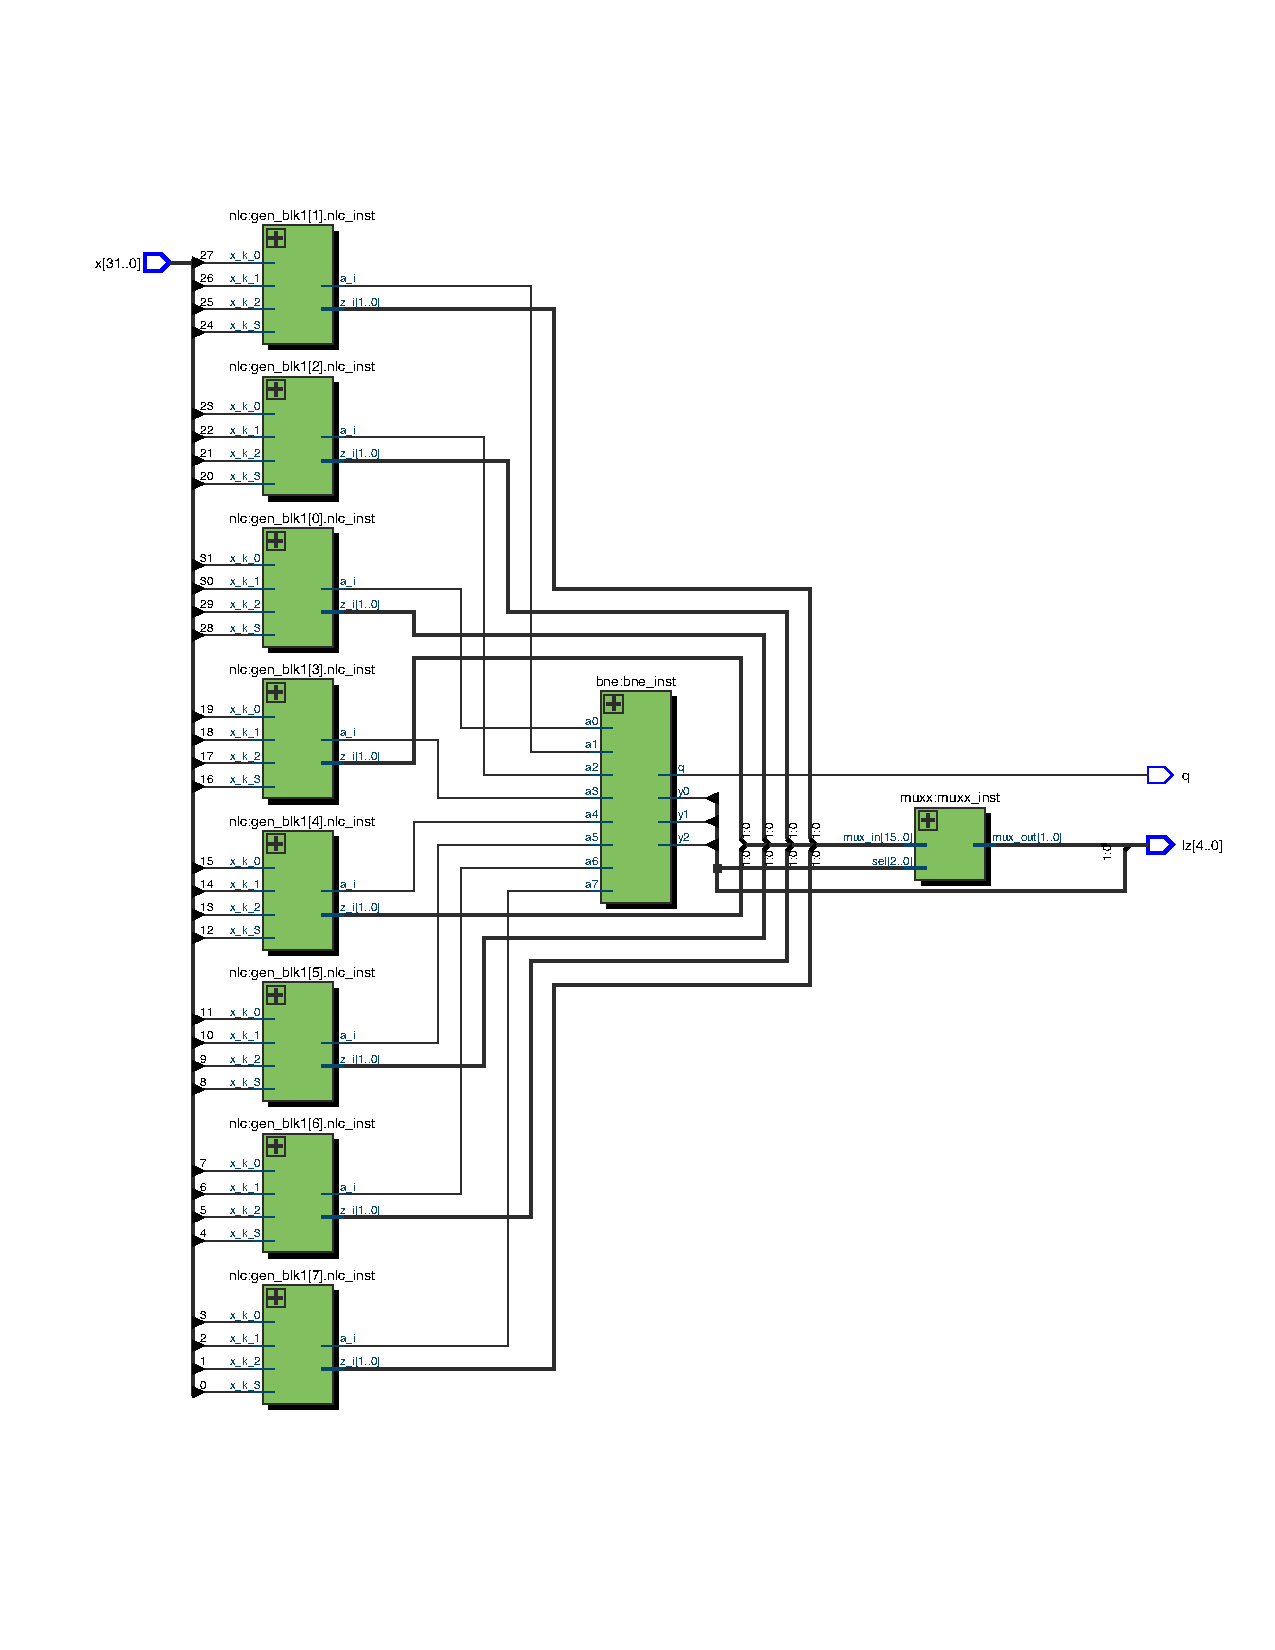
\includegraphics[width=\textwidth]{figures/milenkovic_quartus1.pdf}
\end{figure}

\begin{figure}
    \centering
    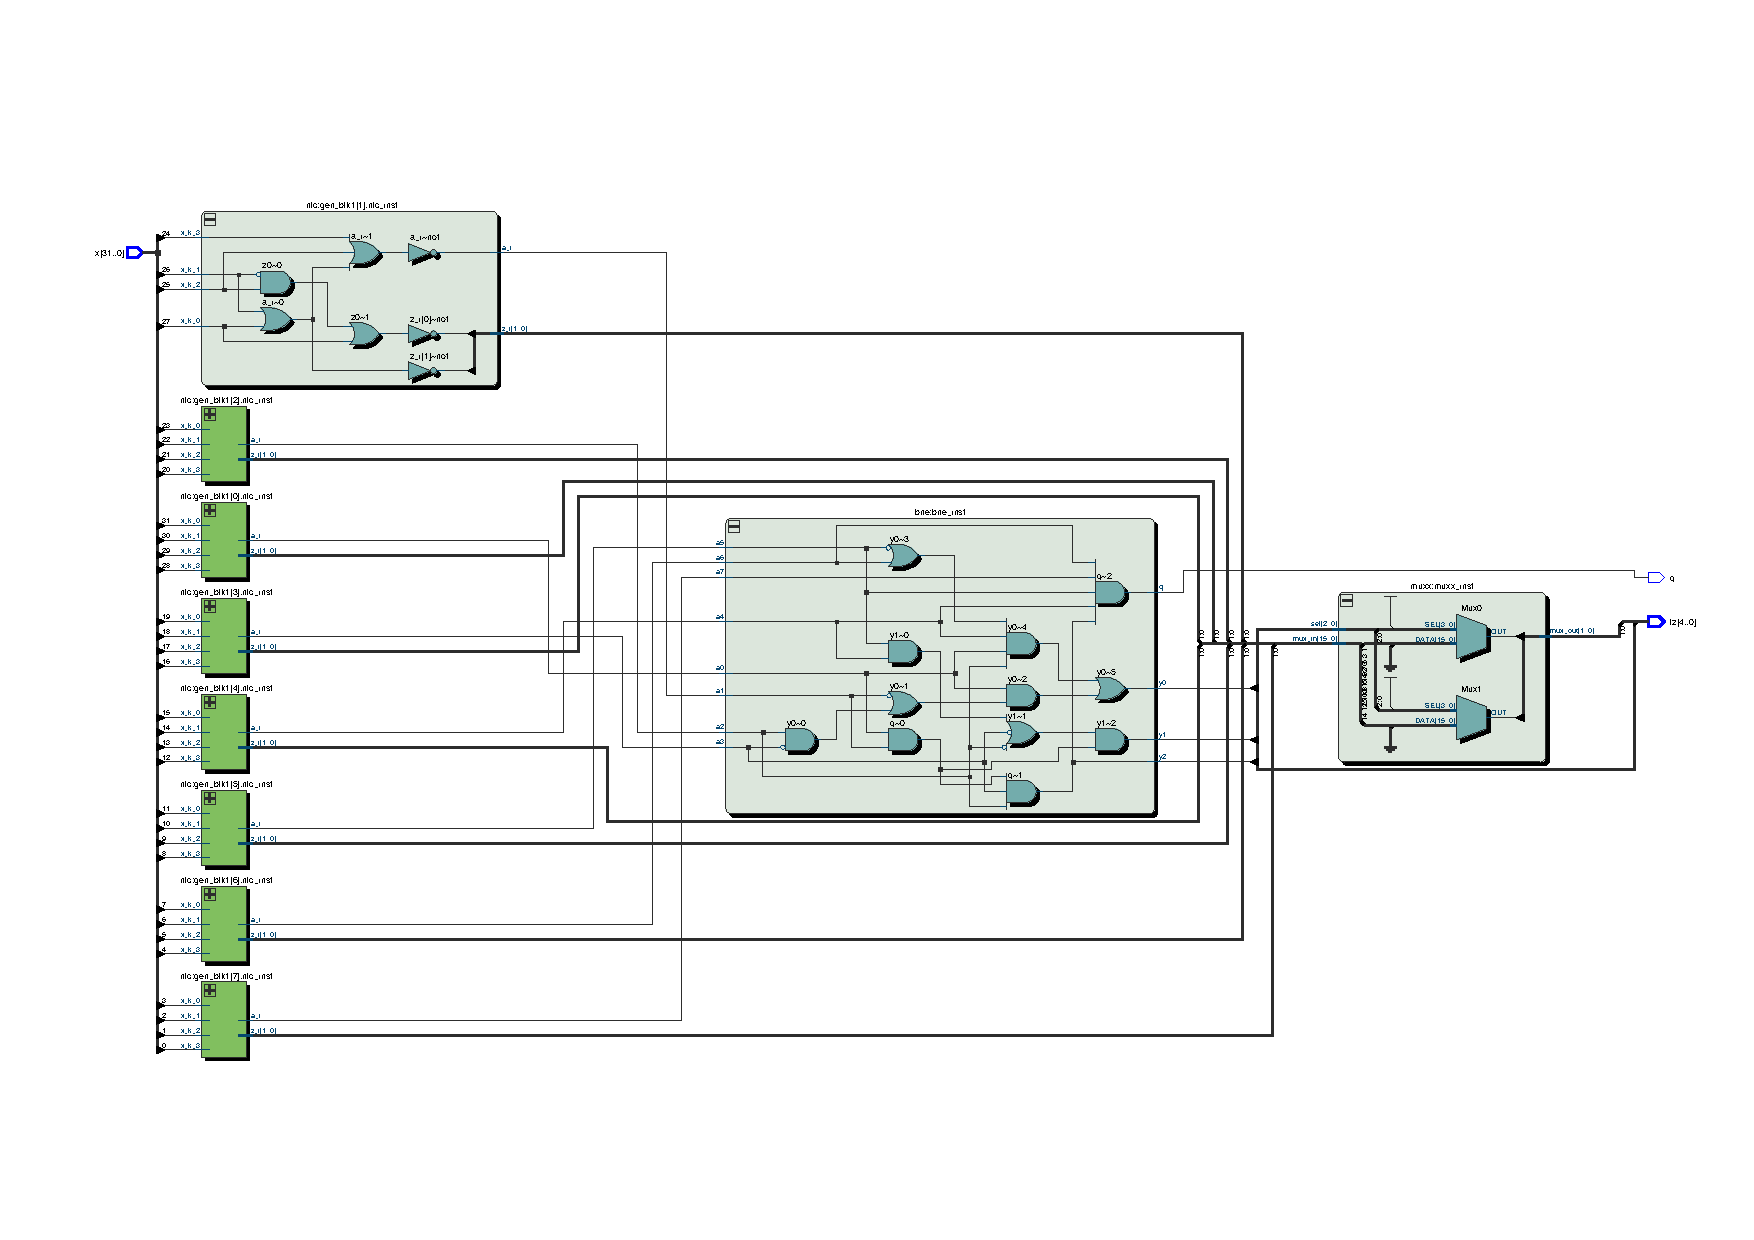
\includegraphics[width=\textwidth]{figures/milenkovic_quartus2.pdf}
    \caption{\cite{milenkovic_modular_2015}'s 16-bits LZC generated schematic}
    \label{fig:milenkovic_lzc_quartus}
\end{figure}


A similar design is presented in \cite{dimitrakopoulos_low-power_2008}, which proposes a semi-tree-based approach elaborating on 16 bits at a time. Like the previous design, this can be extended to other powers of $2$ input bits configurations.

\paragraph{Pacogen LZC}

Another design was proposed in \cite{PACoGen}.
Here, the same basic building block is recursively instantiated, terminating in a simple \textit{and} / \textit{or} gates pair, which make up the base case (figure \ref{fig:pacogen_LOD2_1}).
The truth table (\ref{table:lod21_truth_table}) of \ref{fig:pacogen_LOD2_1} indicates that, at the lowest level, $k$ counts the number of zeros from the left. A sequence without bit alternation is considered invalid, as the $\text{vld}$ flags reports.

The higher-level hierarchical block for the bits $(4:2)$ is shown in Figure \ref{fig:lod42_00001} and consists of two instances of \ref{fig:pacogen_LOD2_1} together with a \textit{or} gate and a multiplexer that routes out the correct $k$ from the ``child" instance, left-wise padded with either a $0$ or $1$.

The truth Table gives an idea about how \ref{table:lod21_truth_table} extends onwards.
\begin{table}[h!]
\centering
    \begin{minipage}{0.5\linewidth}
        \centering
        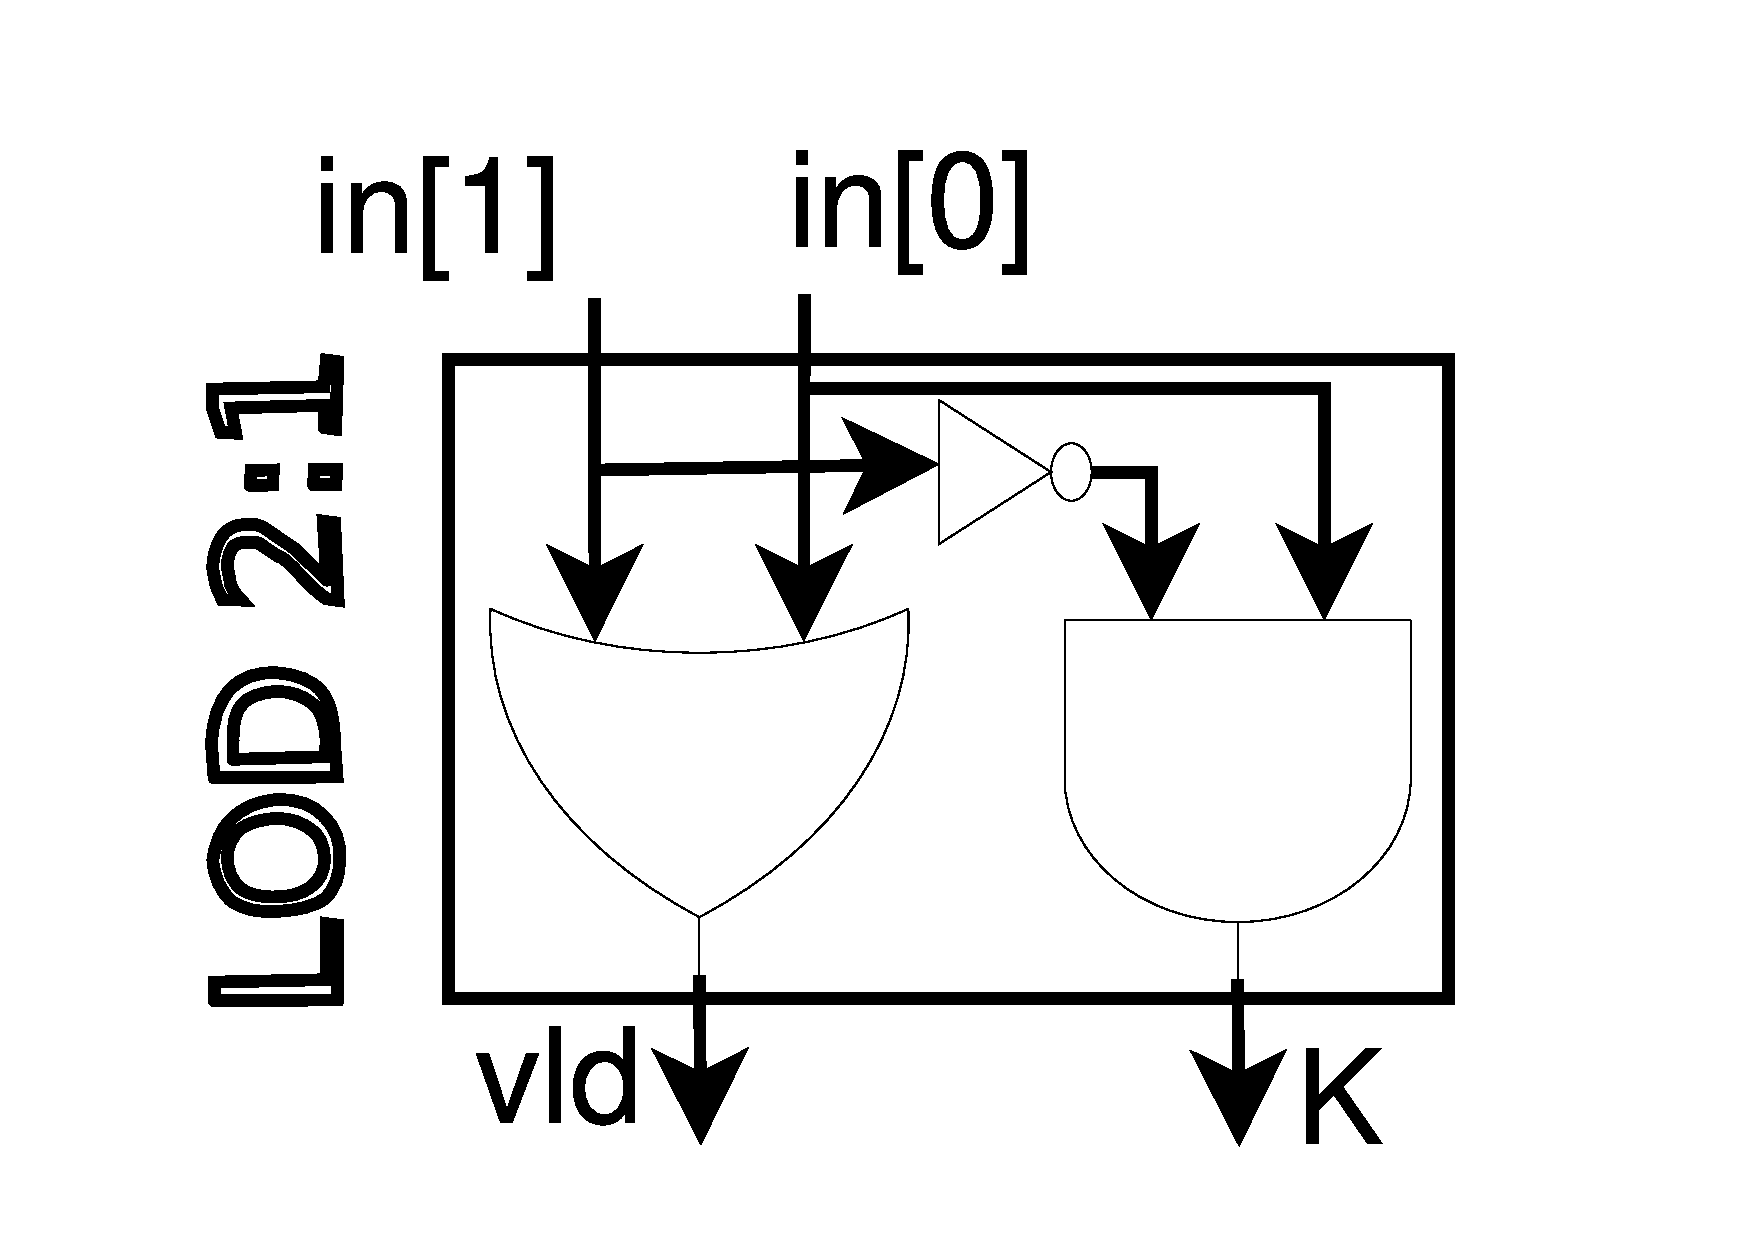
\includegraphics[
            %scale=1
            width=0.85\linewidth]{figures/lod2_1.pdf}
        \captionof{figure}{\cite{PACoGen}'s LOD 2:1 block}
        \label{fig:pacogen_LOD2_1}
    \end{minipage}\hfill
    \begin{minipage}{0.5\linewidth}
        \centering
        \begin{tabular}{cccc}
            \toprule
            \multicolumn{2}{c}{in} & vld & k \\
            \cmidrule{1-2} %\cmidrule{3-3} \cmidrule{4-4}
            0 & 0 & \textbf{0} & 0 \\
            0 & 1 & 1 & 1 \\
            1 & 0 & 1 & 0 \\
            1 & 1 & 1 & 0 \\
            \bottomrule
        \end{tabular}
        \captionof{table}{LOD 2:1 truth table}
        \label{table:lod21_truth_table}
    \end{minipage}
\end{table}

\begin{figure}[h!]
    \begin{minipage}[b]{0.5\linewidth}
        \iffalse
        \centering
        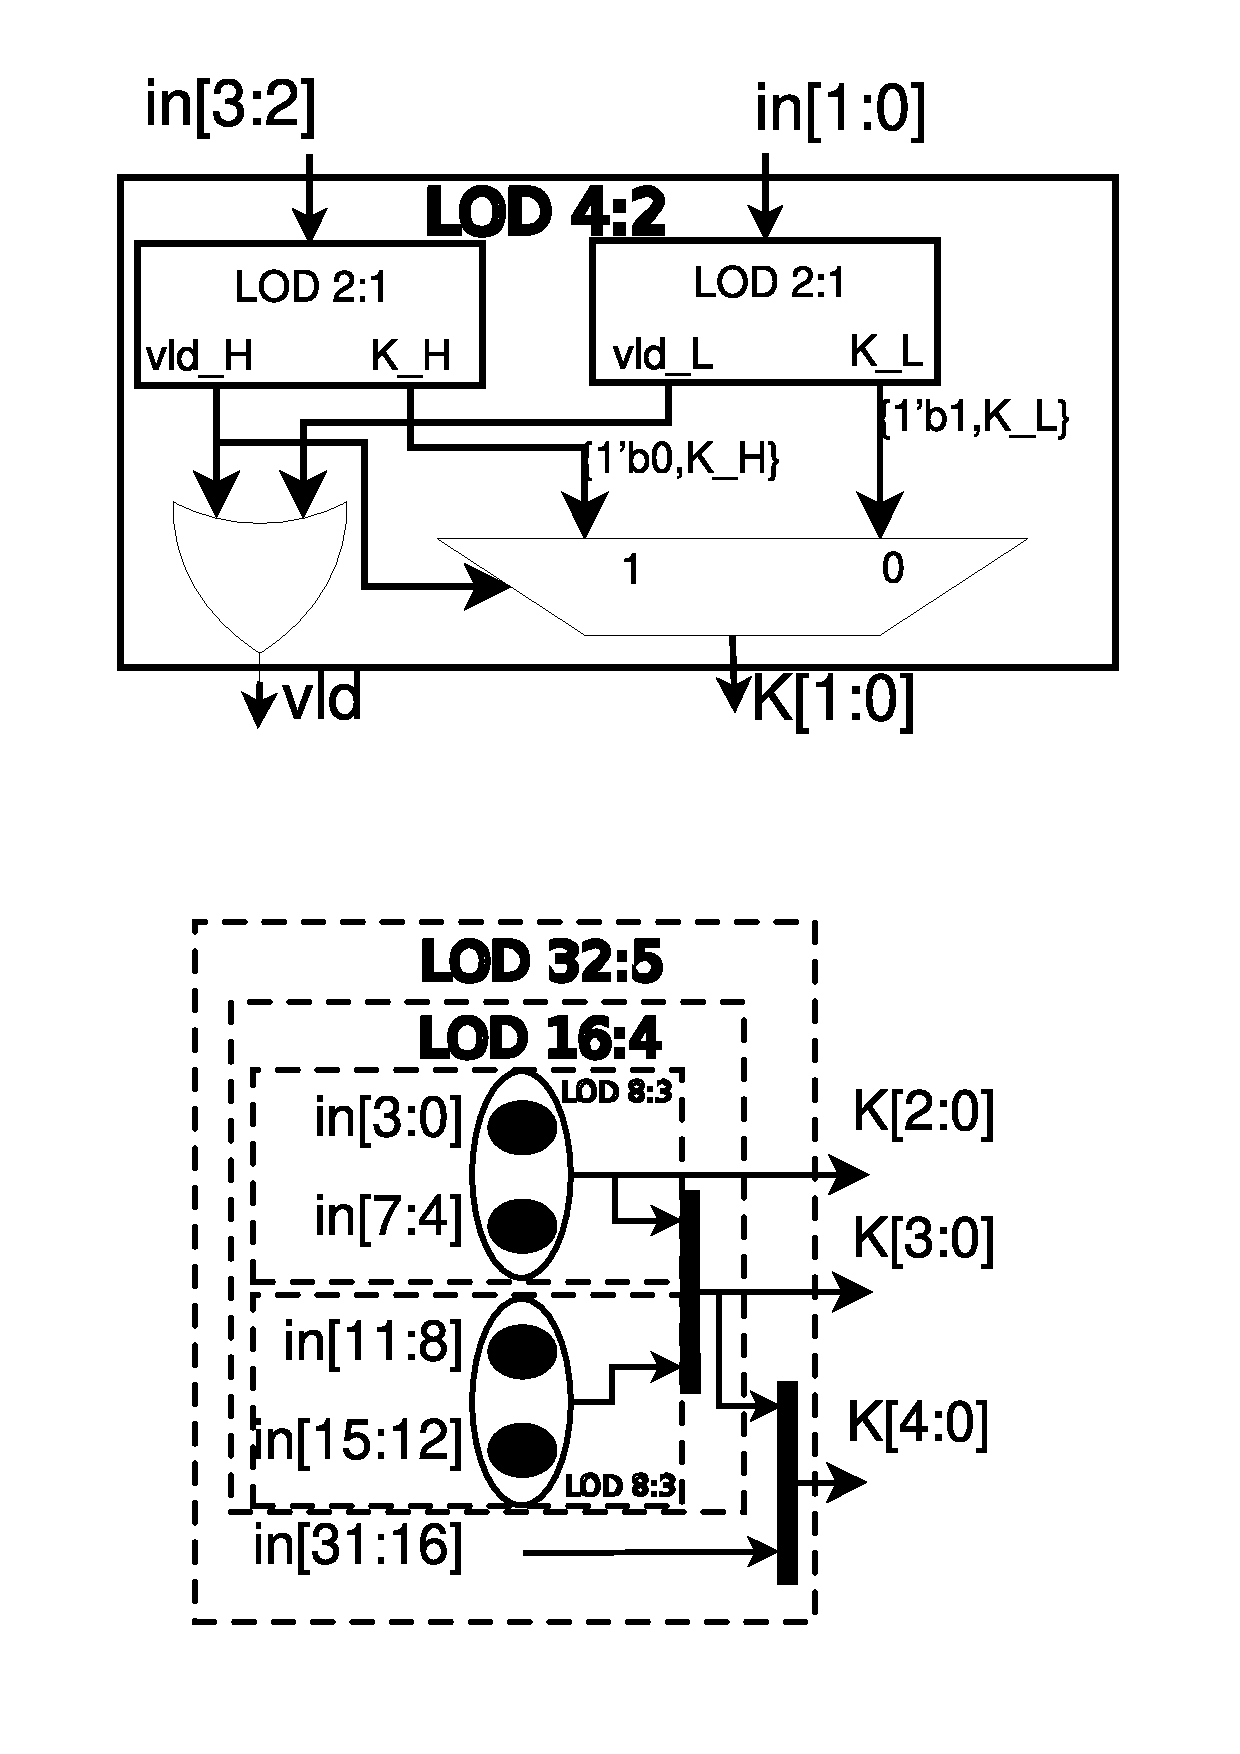
\includegraphics[
            %scale=1
            width=0.8\linewidth,
            valign=t]{figures/pacogen_LODS.pdf}
        \captionof{figure}{\cite{PACoGen}'s LZC architectural building blocks}
        \label{fig:pacogen_LOD_arch}
        \fi

        \centering
        \begin{minipage}{0.6\textwidth}
            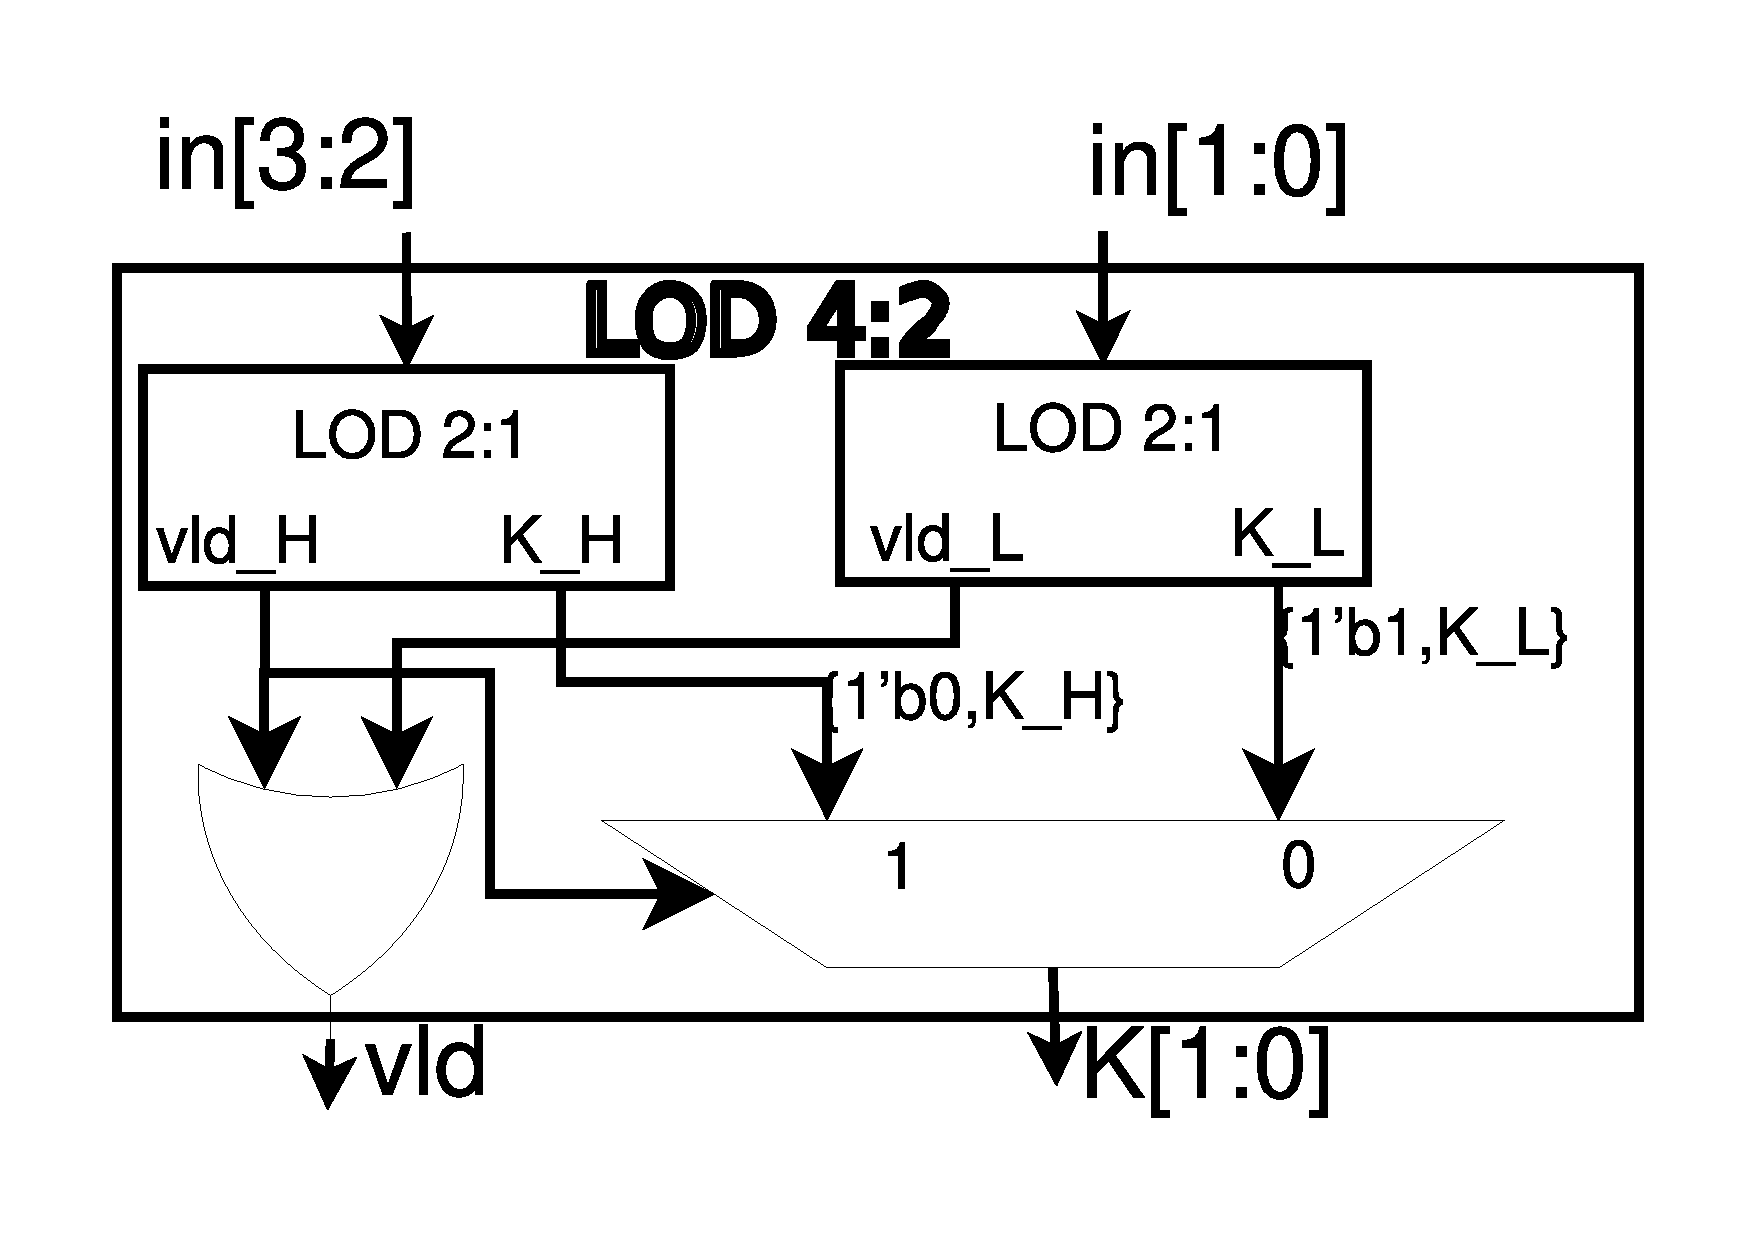
\includegraphics[width=\textwidth]{figures/lod4_2.pdf}
            \caption{LOD 4:2 block}
            \label{fig:lod42_00001}
        \end{minipage}
        \vfill
        \begin{minipage}{0.6\textwidth}
            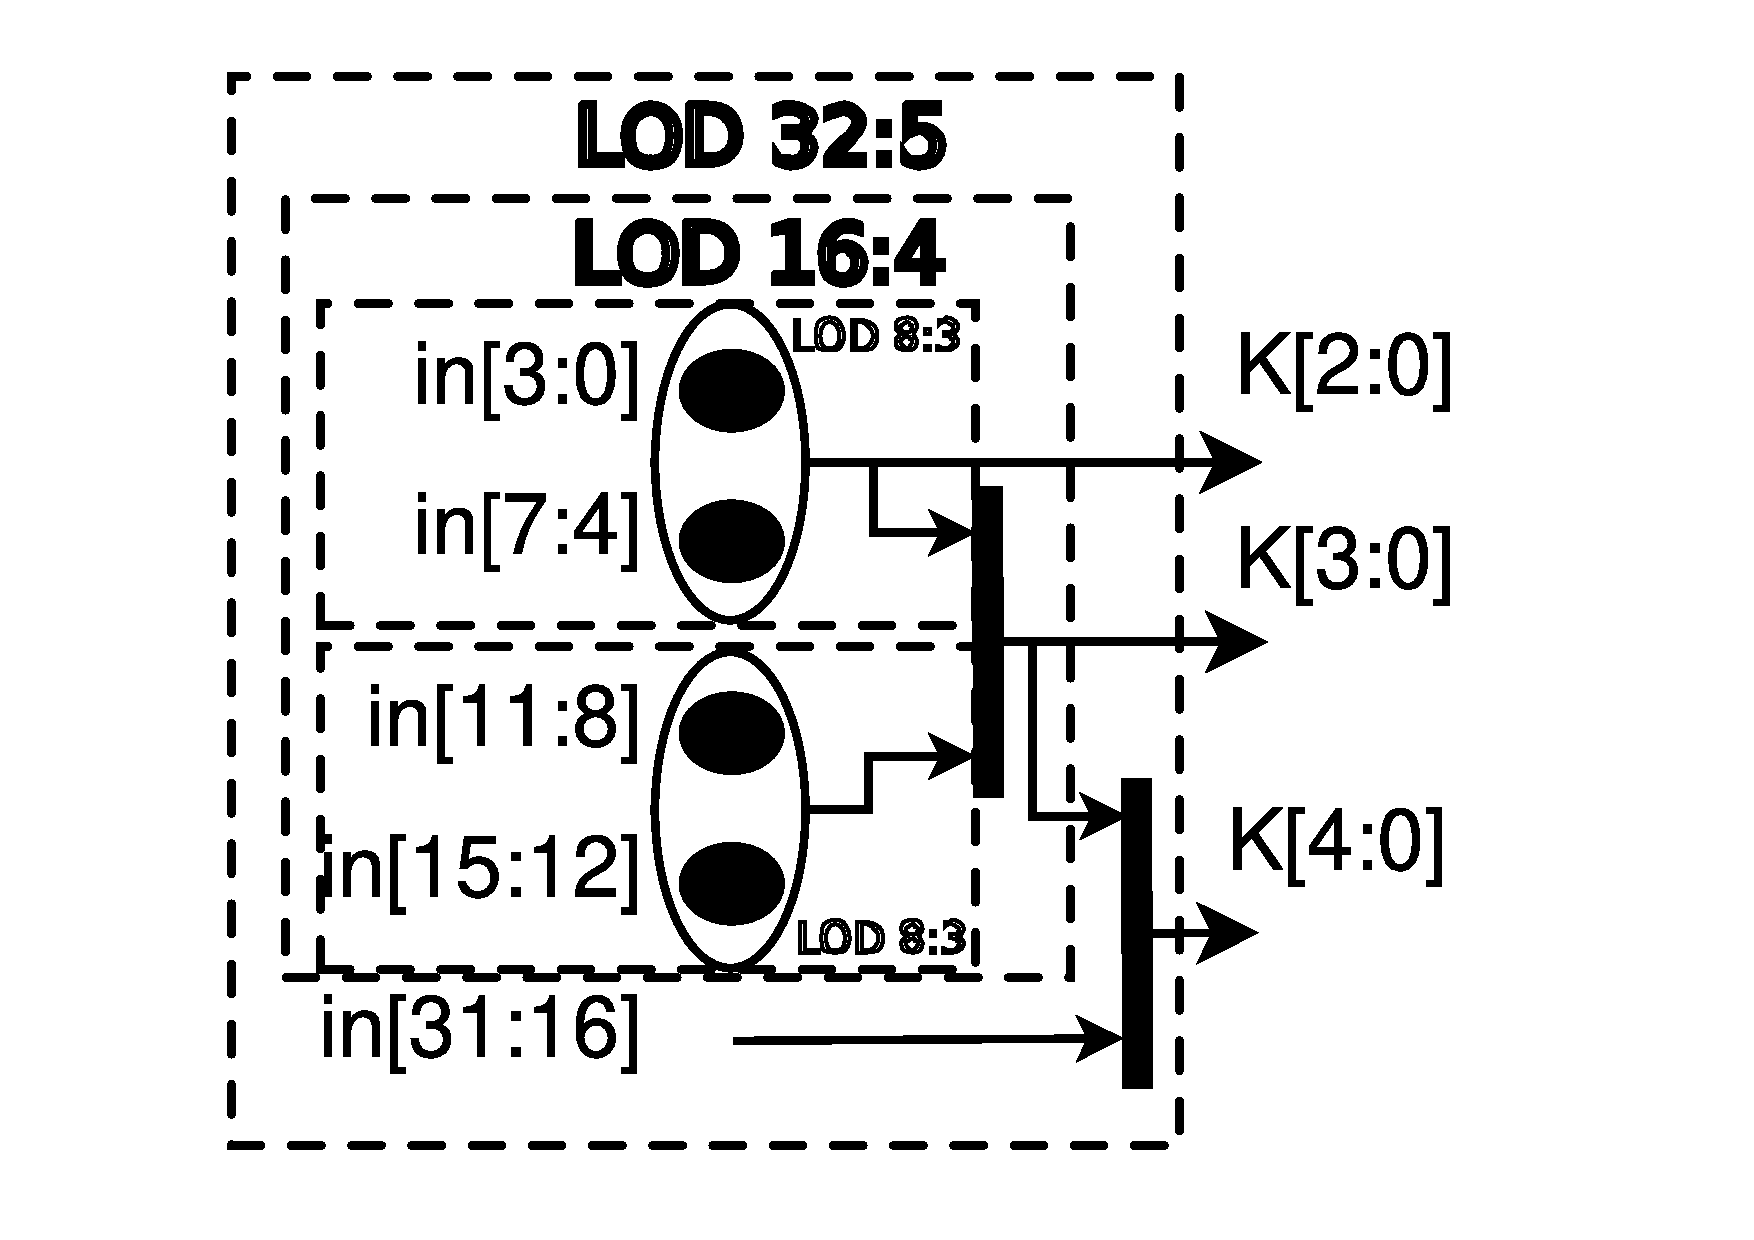
\includegraphics[width=\textwidth]{figures/lod32_5.pdf}
            \caption{LOD 32:5 block}
            \label{fig:lod16_4_0000}
        \end{minipage}
        \captionof{figure}{\cite{PACoGen}'s LZC architectural building blocks}
        \label{fig:pacogen_LOD_arch}
    \end{minipage}
    %
    \begin{minipage}[b]{0.5\linewidth}
        \centering
        \begin{tabular}{cccccccccc}
        \toprule
        \multicolumn{4}{c}{in} & $\text{vld}_l$ & $\text{vld}_h$ & vld & $\text{k}_l$ & $\text{k}_h$ & k \\
        \cmidrule{1-4} %\cmidrule{5-5} \cmidrule{6-6} \cmidrule{7-7} \cmidrule{8-8} \cmidrule{9-9}
        0 & 0 & 0 & 0 & 0 & 0 & \textbf{0} & 0 & 0 & 10 \\
        0 & 0 & 0 & 1 & 1 & 0 & 1 & 0 & 1 & 11 \\
        0 & 0 & 1 & 0 & 1 & 0 & 1 & 0 & 0 & 10 \\
        0 & 0 & 1 & 1 & 1 & 0 & 1 & 0 & 0 & 10 \\
        0 & 1 & 0 & 0 & 0 & 1 & 1 & 1 & 0 & 01 \\
        0 & 1 & 0 & 1 & 1 & 1 & 1 & 1 & 1 & 01 \\
        0 & 1 & 1 & 0 & 1 & 1 & 1 & 1 & 0 & 01 \\
        0 & 1 & 1 & 1 & 1 & 1 & 1 & 1 & 0 & 01 \\
        1 & 0 & 0 & 0 & 0 & 1 & 1 & 0 & 0 & 00 \\
        1 & 0 & 0 & 1 & 1 & 1 & 1 & 0 & 1 & 00 \\
        1 & 0 & 1 & 0 & 1 & 1 & 1 & 0 & 0 & 00 \\
        1 & 0 & 1 & 1 & 1 & 1 & 1 & 0 & 0 & 00 \\
        1 & 1 & 0 & 0 & 0 & 1 & 1 & 0 & 0 & 00 \\
        1 & 1 & 0 & 1 & 1 & 1 & 1 & 0 & 1 & 00 \\
        1 & 1 & 1 & 0 & 1 & 1 & 1 & 0 & 0 & 00 \\
        1 & 1 & 1 & 1 & 1 & 1 & 1 & 0 & 0 & 00 \\
        \bottomrule
        \end{tabular}
        \captionof{table}{LOD 4:2 truth table}
        \label{table:lod42_truth_table}
    \end{minipage}
\end{figure}

Figure \ref{fig:lzc_synthesized} shows the RTL tool-generated schematic of a 16-bits LZC.


\begin{figure}[h!]
    \noindent\makebox[\textwidth]{%
        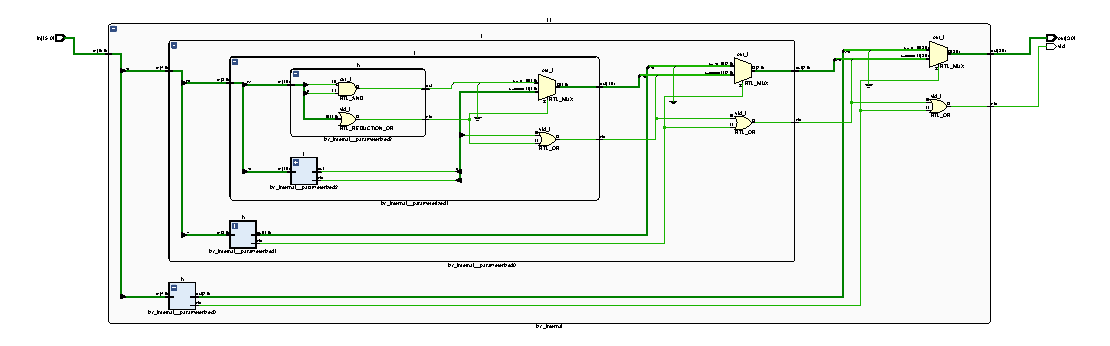
\includegraphics[width=1.3\textwidth]{figures/lzc_pacogen_vivado.pdf}
    }
    \caption{\cite{PACoGen}'s 16-bits LZC generated schematic}
    \label{fig:lzc_synthesized}
\end{figure}







\begin{figure}
    \centering
        \centering
        \includegraphics[width=\textwidth]{figures/core_op.drawio.pdf}
        \caption{\textit{Core op} schematic (conceptual)}
        \label{fig:core_op_ppu_schematic}
\end{figure}   


\begin{figure}
        \centering
        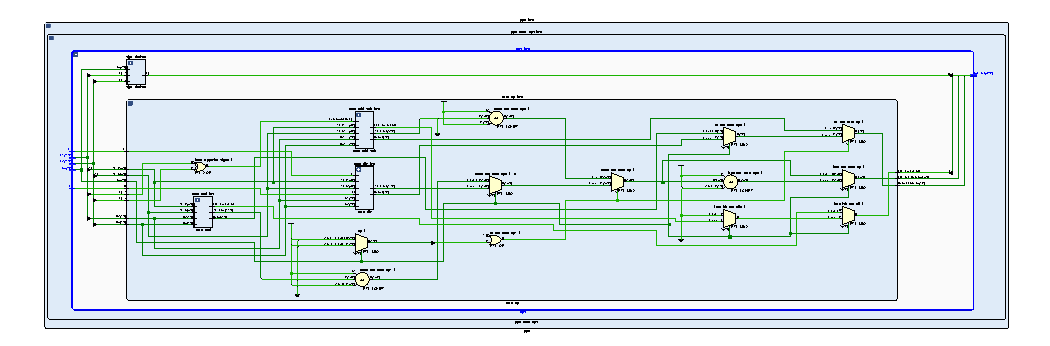
\includegraphics[width=\textwidth]{figures/core_op.vivado.pdf}
        \caption{\textit{Core op} schematic (Vivado)}
        \label{fig:core_op_ppu_schematic_vivado}
\end{figure}   




\subsection{Computation}


The computation stage implements the modules described in Section \ref{sec:posit_ops}.
The input operands are passed as FIR types and the operation is selected by the \textit{op} (short for \textit{operation}) signal.
First, the FIR signal is unpacked in its 3 components (sign, total exponent, and fraction), and the latter two are routed into the submodules. The signs are instead routed into the \textit{sign decisor} module. The involvement of the sign components in the core operations is minimal, as they only indirectly affect the \textit{add/subtract} module which needs the information about whether the signs are even, and some bit-alignments before outputting the newly computed \textit{te} and \textit{frac}.




\subsubsection{Adder/Subtractor}

The adder/subtractor implements the set of operations described in section \ref{sec:posit_ops}. The majority of the steps required for either operation is shared, hence the reason why a common module.
As a consequence of the preliminary \textit{pre-condition} step described in section \ref{sec:posit_extraction}, there is here no need to perform any operation to determine the final sign: the first operand is the largest in magnitude, therefore its sign will determine the output's as well. This consideration saves quite some logic.

The fractions are left shifted by a safe\footnote{\texttt{MAX\_TE\_DIFF}: size such that, if the second operand fraction had to be shifted left by the largest total exponent difference, no bits would be lost} constant amount and the second operand fraction is shifted right back by the difference of the total exponents, such that their \textit{effective exponent} is even and fractions are weighted equally.
Next, the fractions are added/subtracted together -- depending on the \textit{have opposite sign} flag -- before being routed into the \textit{core add} and \textit{core sub} sub-modules. Those implement the steps that differ between the two: the addition module needs to detect whether fraction overflow ($f \ge 2.0$) has occurred\footnote{recall that  that $(1.f_1) + [(1.f_2) \cdot 2^{-b}] \in [1.0, 4.0) \equiv [1.0, 3.999\dots]$, i.e. the integer part of the resulting fraction will, at most, occupy $\lceil\log_2(3)\rceil = 2$ bits} and fix that; the subtraction module needs to do the symmetrical operation, i.e. detect fraction underflow ($f < 1.0$) and fix that.

Fixing an overflow is simple: the fraction is shifted right by $1$, in order to obtain the canonical fraction format again, and the exponent is adjusted with an increment\footnote{e.g.: $10.010 \cdot 2^{\epsilon} \equiv (1.001 \cdot 2^1) \cdot 2^{\epsilon} \equiv 1.001 \cdot 2^{\epsilon + 1}$}. Shifting the fraction right, however, can introduce inaccuracies: the least significant bit can be a $1$ and information about whether truncation occurred must be preserved and forward-propagated in order to get the subsequent rounding right.

Fixing an underflow, must be carefully approached:
the resulting fraction\footnote{$(1.f_1) - [(1.f_2) \cdot 2^{-b}] \in [0.0, 2.0) \equiv [0.0, 1.999\dots]$} can span from
% $0$ to $1.999\dots$ -- i.e.
$(1.f) \cdot 2^{-\infty}$ to $(1.f) \cdot 2^{0}$; this means that an arbitrary number of zeros can precede the $1$ that can constitute the most significant bit of a fraction.
This is the ideal place where the second instance of the LZC presented in Figure \ref{fig:lzc_synthesized} can be used.
The figure returned by the LZC module is used to shift the fraction back to its canonical form, and, at the same time, to simultaneously update the total exponent difference.

The parent module -- called \textit{core add/sub} -- selects, using the \textit{have same sign} flag, the correct (total exponent, fraction) pair, together with the \textit{is truncated} flag for later correct rounding computation.

\begin{figure}
    \centering
    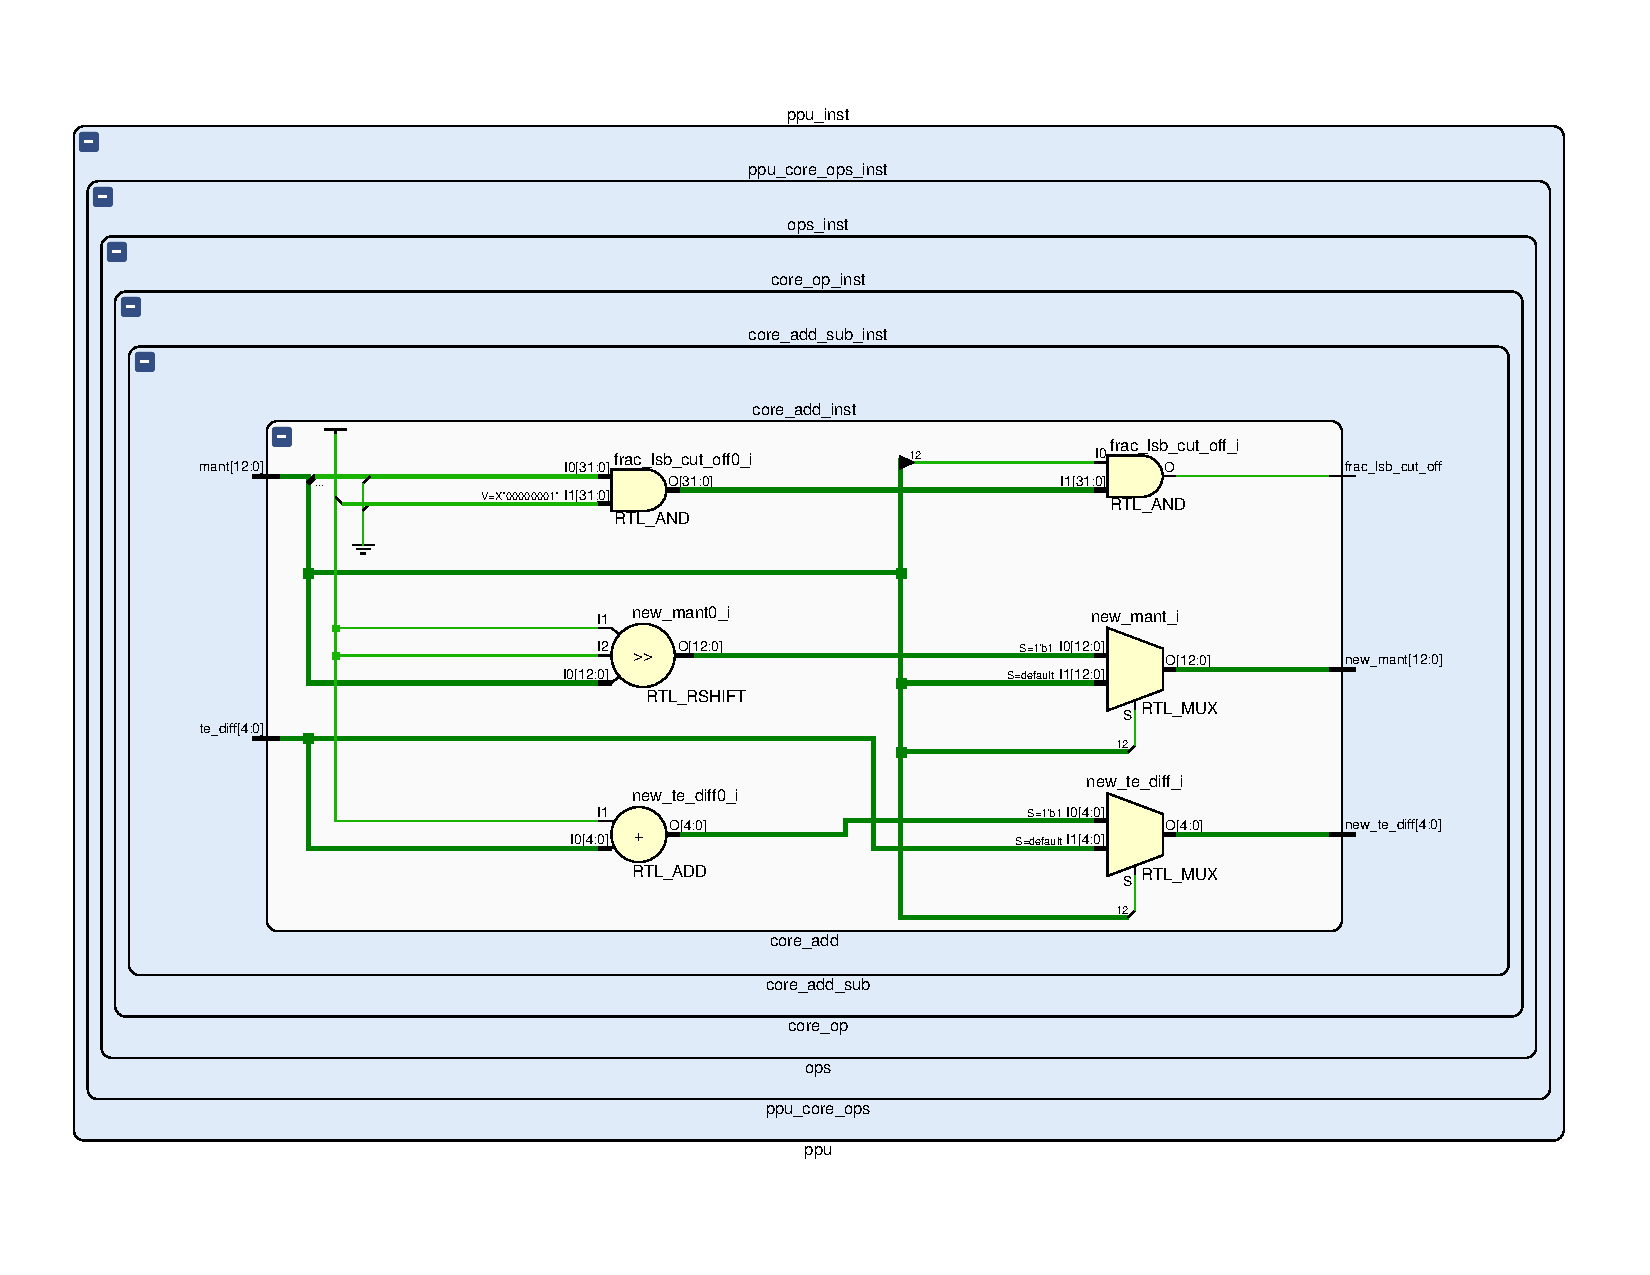
\includegraphics[width=\textwidth]{figures/core_add_vivado.pdf}
    \caption{\textit{Core add} (Vivado)}
    \label{fig:core_add_vivado}
\end{figure}%
\begin{figure}
    \centering
    \includegraphics[width=\textwidth]{figures/add-sub-core.drawio.pdf}
    \caption{\textit{Core add/sub} (conceptual)}
    \label{fig:core_add_sub_schematic_conc}
\end{figure}%

\begin{figure}
    \centering
    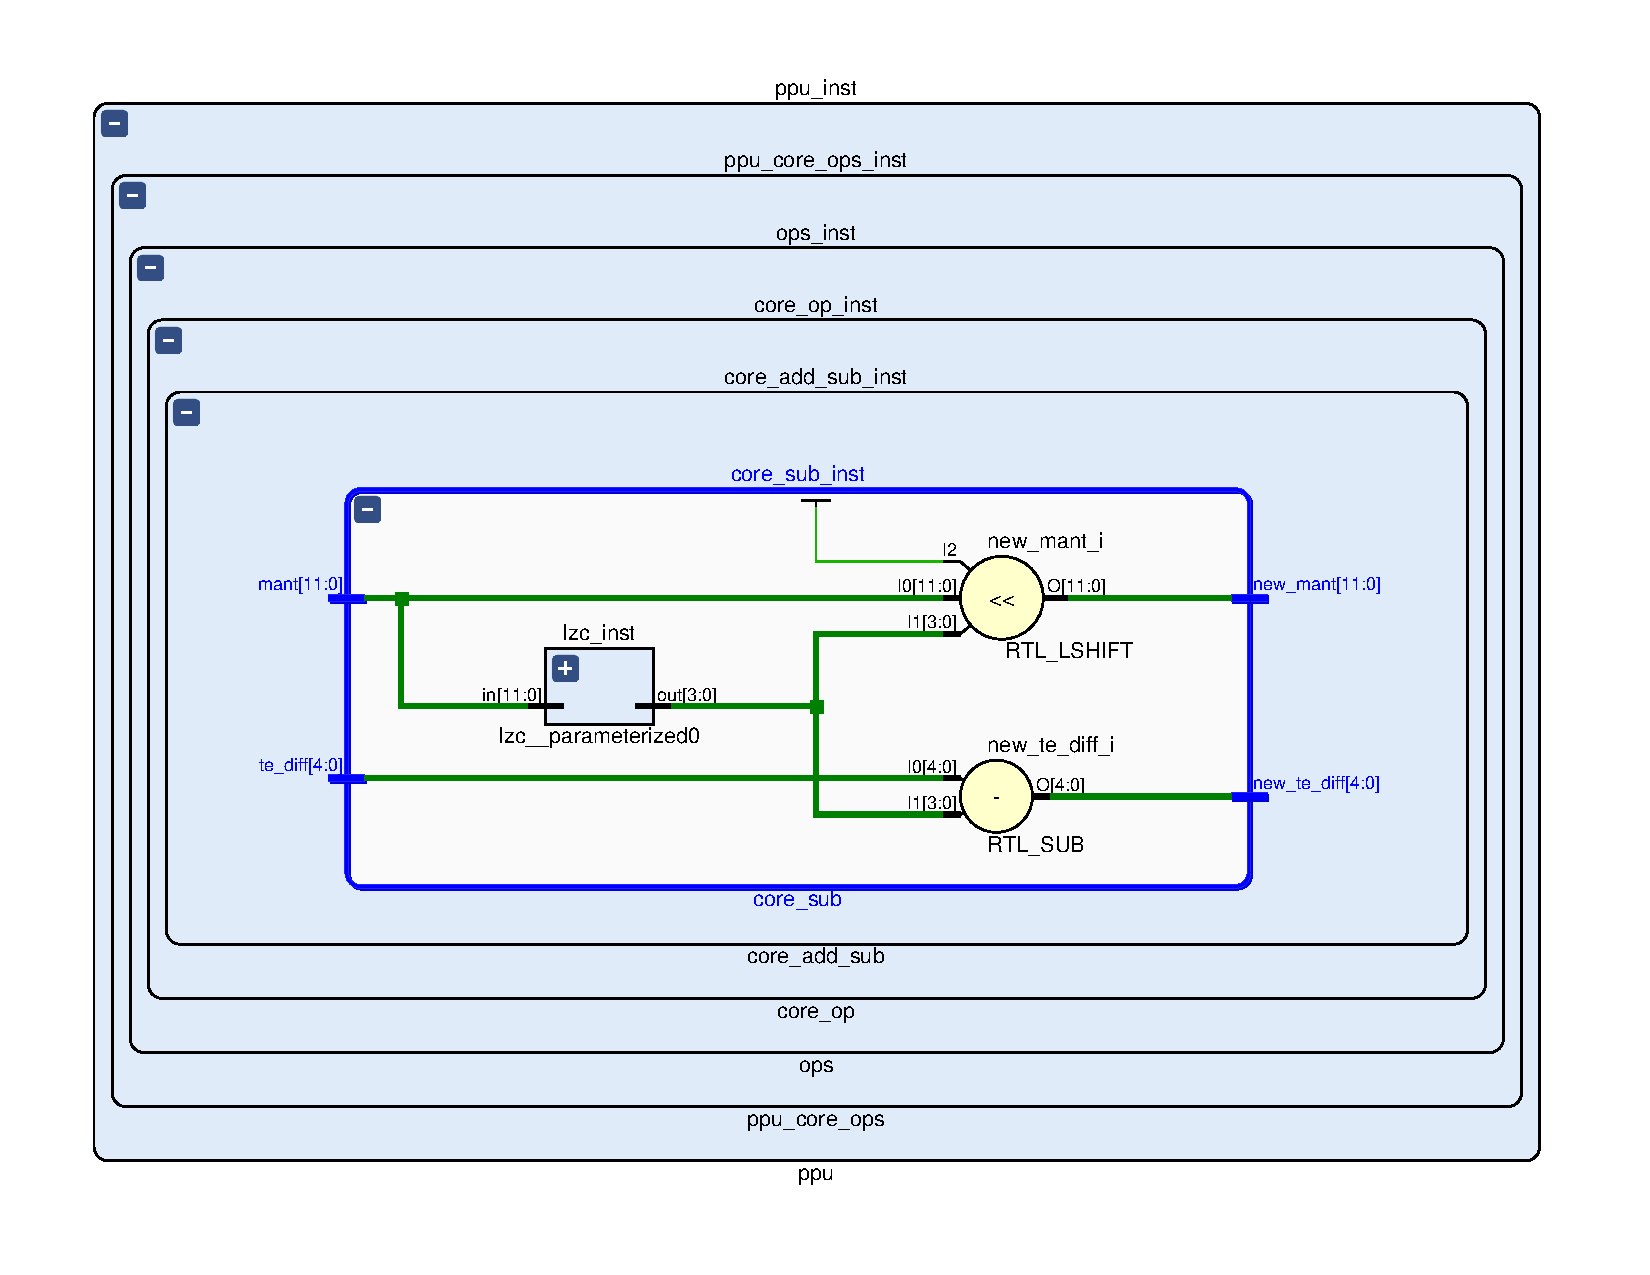
\includegraphics[width=1\textwidth]{figures/core_sub_vivado.pdf}
    \caption{\textit{Core sub} (Vivado)}
    \label{fig:core_sub_vivado}
\end{figure}

\begin{figure}
    \centering
    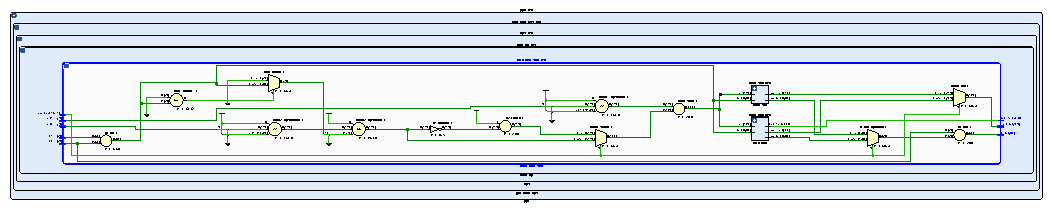
\includegraphics[width=1\textwidth]{figures/core_add_sub_vivado.pdf}
    \caption{\textit{Core add/sub} (Vivado)}
    \label{fig:core_add_sub_vivado}
\end{figure}%




\subsubsection{Multiplier}

\begin{figure}
    \centering
    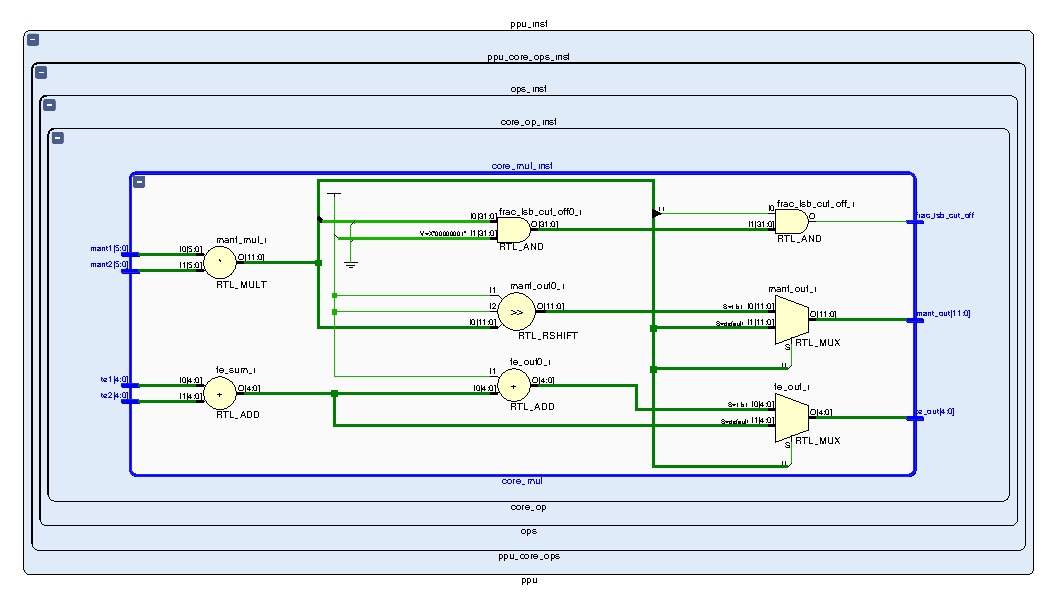
\includegraphics[width=\textwidth]{figures/mul_vivado.pdf}
    \caption{\textit{Core multiplier schematic} (Vivado)}
    \label{fig:mul_vivado}
\end{figure}


The multiplier handles the production of the two fractional components of the operands and sums their total exponents (\textit{te}). Similarly to the addition, fraction overflow can occur: in this case, a flag \textit{is truncated} is used to notify whether the least significant bit is a $1$. The fraction is shifted right by 1 in the canonical form and the total exponent is incremented by 1 to adjust the fraction shift.

The unsigned integer multiplier present in the schematic is inferred by the synthesis tool. 
% \hl{check}
%





\subsubsection{Divider}\label{divider_hardware_ppu}

% \hl{reformulate if time allows}

The core divider module implements the steps described in section \ref{Approximated_Algorithms}.

Conceptually, the divider scheme is shown in Figure \ref{fig:nr_schematic}.

First, an approximation of the reciprocate of the second operand mantissa is computed using Algorithm \ref{alg:reciprocal_approx_modified_drom} adapted to fixed-point arithmetic.
Next, the output is used as input inside a single Newton-Raphson stage.

With reference to an 8-bit posit division operation, the core divider instance is synthesized as in Figure \ref{fig:div1vivado} and \ref{fig:div2vivado}. We compared the module accuracy with the one presented by \cite{PACoGen} in \ref{table:comparison_div_against_pacogen_table}.

    \begin{figure}
        \includegraphics[width=1\textwidth]{figures/newton_raphson_drawing.drawio.pdf}
        \caption{\textit{Core div} (conceptual)}
        \label{fig:nr_schematic}
    \end{figure}

    \begin{figure}
        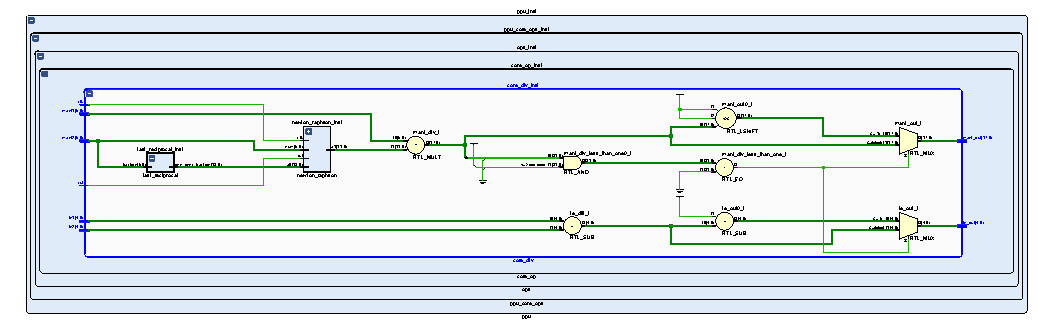
\includegraphics[width=1\textwidth]{figures/div_vivado.pdf}
        \caption{\textit{Core div} (Vivado)}
        \label{fig:div1vivado}
    \end{figure}
    \begin{figure}
        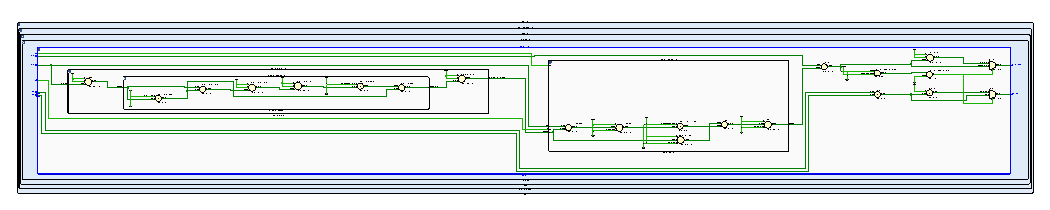
\includegraphics[width=1\textwidth]{figures/div_opened_vivado.pdf}
        \caption{\textit{Core div} opened (Vivado)}
        \label{fig:div2vivado}
    \end{figure}








\subsection{Normalization}

The \textit{normalization} stage rebuilds the posit from the fields output by the computation stage.



\begin{figure}[h!]
    \begin{center}
    \includegraphics[width=1\textwidth]{figures/fir-to-posit-drawing.drawio.pdf}
    \caption{FIR to Posit}
    \label{fig:fir2posit_ppu}
    \end{center}
\end{figure}

The FIR number is unpacked in sign (\texttt{sign}), exponent (\texttt{total\_exp}), and fraction (\texttt{frac\_full}) fields.
\texttt{frac\_full} represent the full fraction, formatted as a \texttt{Fx<0, \_>} fixed-point, without any truncation being applied from the previous (computation) stage.

Within ``pack fields" module the total exponent is separated into $k$ (regime value) and $e$ (exponent value). Hardware-wise this can be implemented with two shifts: \texttt{k = total\_exp >> ES}, \texttt{exp = total\_exp - (k << ES)}, that corresponds to form and remainder of the division of the total exponent by 2.
The value of $k$ determines the regime size and, as a consequence, the remaining fields, including the size of the final fraction. 
The fraction, combined with its final length determines the value of the rounding bits (Guard, Round, Sticky) as brought to the attention in figure \ref{fig:fraction_before_rounding}.

``Posit encoder" combines together the fields into one bit-string, which is the non-rounded posit.
Then, \textit{nearest-even} rounding is applied: this is a simple bit increment on posit based on the logic value of the other input flags.

Lastly, the sign is set: this consists of either no intervention if the resulting posit is meant to represent a positive value (sign = 0), or bit-string two's complement otherwise (sign = 1).



\subsection{Conversions}

% \hl{insert fig simil clarinet}






\begin{figure}[H]
        \centering
        \includegraphics[width=1\textwidth]{figures/top_no_conversions.pdf}
        \caption{\textit{bare} PPU}
\end{figure}
\begin{figure}
        \includegraphics[width=1\textwidth]{figures/top_P2F.pdf}
        \caption{\textit{bare} PPU with support to posit-to-float conversion}
        \label{fig:top_p2f_00000001}
\end{figure}
\begin{figure}
        \includegraphics[width=1\textwidth]{figures/top_all.pdf}
        \caption{\textit{bare} PPU with support to posit-to-float and float-to-posit conversions}
\end{figure}



\begin{figure}[H]
    \centering
    \includegraphics[width=\textwidth]{figures/posit_to_float_and_float_to_posit.pdf}
    \caption{Posit to Float and Float to Posit}
    \label{fig:posittofloatandfloattoposit}
\end{figure}

\begin{table}
\begin{center}
\begin{tabular}{||c c c | c||}
    \hline
    op & $in_1$ & $in_2$ & $out$ \\ [0.5ex]
    \hline\hline
    \texttt{+} & $p_1$ & $p_2$ & $p_1 + p_2$ \\
    \hline
    \texttt{-} & $p_1$ & $p_2$ & $p_1 - p_2$ \\
    \hline
    \texttt{*} & $p_1$ & $p_2$ & $p_1 * p_2$ \\
    \hline
    \texttt{/} & $p_1$ & $p_2$ & $p_1 / p_2$ \\
    \hline
    \texttt{f2p} & $f$ & $-$ & \texttt{f2p}$(f)$ \\
    \hline
    \texttt{p2f} & $-$ & $p$ & \texttt{p2f}$(p)$ \\
    \hline
\end{tabular}
\captionof{table}{PPU operations. $+,\ -,\ \times,\ \div,$ \texttt{f2p}, \texttt{p2f} encoded progressively from \texttt{0b000} to \texttt{0b101}.}
\label{Tab:table_ops_ppu}
\end{center}
\end{table}




\section{Pipelined architecture}\label{pipelined_ppu_section}


The design presented in the previous section was based on a single-stage data path.


\begin{figure}
    \centering
    \includegraphics[width=1\textwidth]{figures/pipeline_drawio1.pdf}
\end{figure}
\begin{figure}
    \includegraphics[width=1\textwidth]{figures/pipeline_drawio2.pdf}
    \caption{Non-pipelined vs pipelined circuit} 
    \label{fig:pipeline_vs_nonpipeline}
\end{figure}

Pipeline-ing is a common technique adopted in digital design and computer architecture to increase the frequency of the computations. In practice we decompose a long combinatory circuit with a delay of $t_{pd_0}$ into several $N$ shorter combinatory circuits that have different delays $t_{pd_1}, \dots t_{pd_{N}}$, each one smaller than $t_{pd_0}$. This helps loosen the \textit{setup} and \textit{hold} time requirements of the hardware registers;  as a consequence, the overall circuit can operate at higher frequencies. The throughput, defined as the inverse of time between two different $d_{out}$ presented on the output, goes from $1/clk_1$ to $1/clk_2$, and increases according to it.
The latency, on the other hand, defined as the time it takes for a given input to traverse the sequence and turn up on the output, alters from $1/clk_1$ to $N \cdot (1/clk_2)$, which may be larger or smaller than the initial one

With reference to Figure \ref{fig:pipeline_vs_nonpipeline}, the \textit{speedup} is defined as\footnote{\cite{lilja_pipelining_2004} $speedup = T_{non-pipelined}/T_{pipelined}$} equation\footnote{$t_{cq}$ (clock-to-q delay) and $t_{su}$ (setup time) are technology-dependent parameters} \eqref{equ:speedup_equation2},
        \begin{equation}\label{equ:speedup_equation2}
            \begin{aligned}
                speedup &= \frac{1/f_{clk_1}}{1/f_{clk_2}} \\
                &= \frac{f_{clk_2}}{f_{clk_1}} = \\
                &= \dfrac{\dfrac{1}{t_{cq} + t_{su} + \max\{t_{pd_1}, \dots, t_{pd_N} \}}}{\dfrac{1}{t_{cq} + t_{su} + t_{pd_0}}} = \\
                &= \frac{t_{cq} + t_{su} + t_{pd_0}}{t_{cq} + t_{su} + \max\{t_{pd_1}, \dots, t_{pd_N} \}}
            \end{aligned}
        \end{equation}
    %
        \begin{figure}
            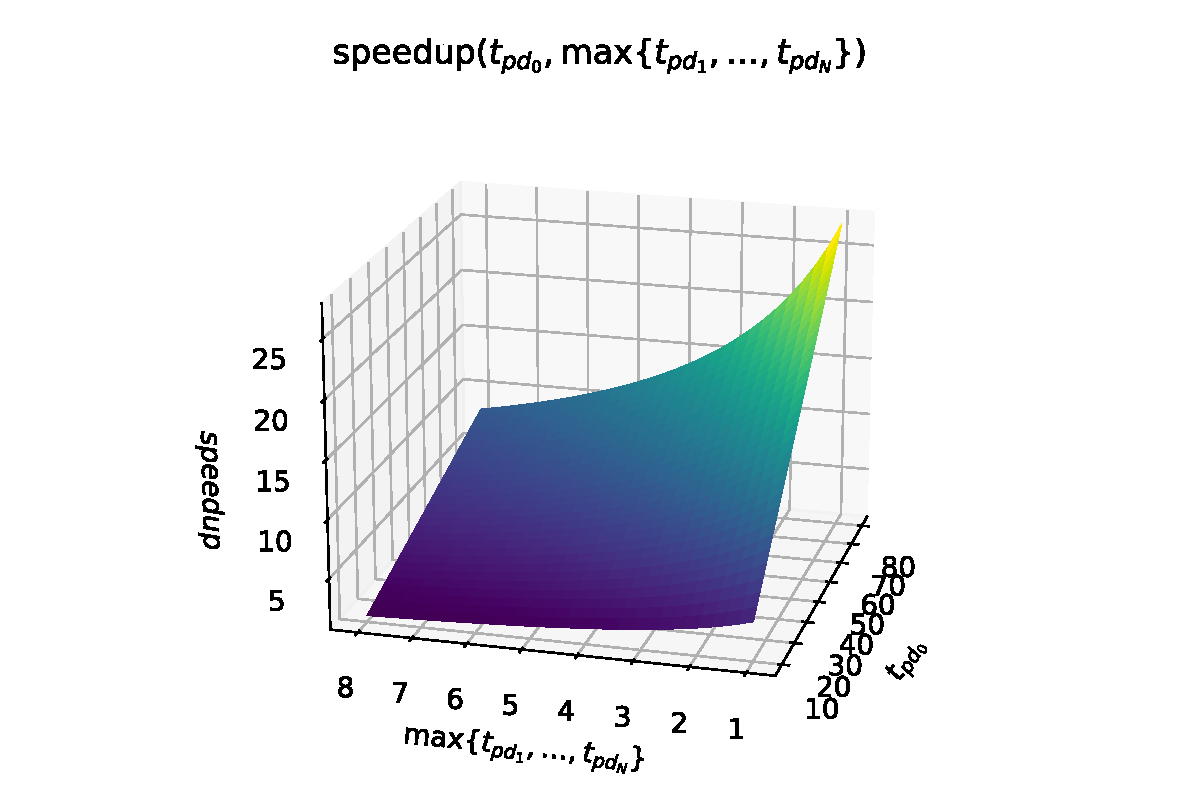
\includegraphics[width=1\textwidth]{figures/3d_plot_speedup.pdf}
            \captionof{figure}{Pipelining speedup}
            \label{fig:speedupplot}
        \end{figure}


As a first step of the pipelined PPU, we separated the combinatory path between each top level stage: we put one registers block between the \textit{extraction} and \textit{operations} stages, and another one between \textit{operations} and \textit{normalization} stage (Figure \ref{fig:top_p2f_00000001}  $\rightarrow$ \ref{fig:top_all_PL2}).

In the second step, we add a register block inside the \textit{computation} module -- specifically, the core divider; this  enabled us to break the critical path inside the divider unit. This critical path was due to the \textit{fast reciprocate} + \textit{Netwon Raphson} combinatorial circuit (Figure \ref{fig:top_all_PL3}).



Since we introduce a non-homogeneous subdivision of stages across the different modules, we needed to orchestrate the different stages with a specific control unit.



\begin{figure}
    \centering
    \includegraphics[width=\textwidth]{figures/pipeline_ops_diagram1.pdf}
    \caption{Timing diagram of posit operations without pipelining}
    \label{fig:timing_diagram_4_stagesdiv_3stagesothers_without_pipelining}
\end{figure}
\begin{figure}
    \centering
    \includegraphics[width=\textwidth]{figures/pipeline_ops_diagram2.pdf}
    \caption{Timing diagram of posit operations with pipelining}
    \label{fig:timing_diagram_4_stagesdiv_3stagesothers_with_pipelining}
\end{figure}



The timing diagram in Figure \ref{fig:timing_diagram_4_stagesdiv_3stagesothers_with_pipelining}  better explains the previous statement: each \textit{non-div} operation in the pipeline traverses  the three \textit{execution}-\textit{computation}-\textit{normalization} (E-C-N) stages; meanwhile, a  \textit{div} operation also traverses the two sub-stages (C1, C2) inside the \textit{computation} stage.

It is clear that for each transition from a \textit{non-div} to a \textit{div} operation we need to ignore the output for one cycle: this comes from \textit{div} having one additional stage in the pipeline.

On the other hand, a transition from a \textit{div} to a  \textit{non-div} operation requires the \textit{non-div} operation to stall its execution. E and C would be able to run concurrently, however, the normalization stage would conflict with the previous operation. Stalling the execution -- anytime before the conflict -- is the conventional way to go around this.


With these asymmetries we required a proper control unit running a finite state machine able to control the \textit{div}-\textit{non-div} (and vice-versa) transitions, emitting \textit{stall} and \textit{valid-output} signals to the core PPU and output respectively.

To mitigate this circumstance we can adopt two different: the first is a compiler modification that involves intercepting the transitions from \textit{div} to \textit{non-div} and interposing a \texttt{nop} instruction.

The second solution consists in slowing down the rest of the operations by one cycle, obtaining the same number of cycles for every operation in the PPU.






\begin{figure}
\centering
    \includegraphics[width=1\textwidth]{figures/top_all_PL2.pdf}
    \caption{3-stage pipelined PPU}
    \label{fig:top_all_PL2}
\end{figure}
\begin{figure}
\centering
    \includegraphics[width=1\textwidth]{figures/top_all_PL3.pdf}
    \caption{4-stage pipelined PPU}
    \label{fig:top_all_PL3}
\end{figure}


\begin{figure}[h!]
    \centering
    \includegraphics[width=1\textwidth]{figures/ppu_all_with_control_unit_3a.pdf}
    \caption{4-stage div, 3-stage add/sub/mul. Control unit issues \textit{stall} signals to the core PPU}
    \label{fig:ppu_with_control_unit1}
\end{figure}%
 
\begin{figure}
    \centering
    \includegraphics[width=1\textwidth]{figures/ppu_all_with_control_unit_3b.pdf}
        \caption{4-stage operations. Control unit only asserts \textit{valid\_out}}
        \label{fig:ppu_with_control_unit2}
\end{figure}%

\begin{figure}
    \centering
    \includegraphics[width=1\textwidth]{figures/simple_fsm.pdf}
    \caption{Simple Finite State Machine}
    \label{fig:simple_fsm}
\end{figure}



Plots in Figures \ref{fig:spartan7_stages_vs_freqlatency_64_32_8_2} and \ref{fig:spartan7_stages_vs_freqlatency_64_64_16_2} show the variations of highest frequency/lowest latency achievable as the number of pipeline stages increases\footnote{specifically, moves from no pipeline to 3 and 4 stages, as described}, on a Spartan7 \texttt{xa7s6cpga196-2I} FPGA device, in two different configurations: figure \ref{fig:spartan7_stages_vs_freqlatency_64_32_8_2} is referred to a  PPU core supporting $P\langle8,2\rangle$ posits + conversions to single-precision floating point, figure \ref{fig:spartan7_stages_vs_freqlatency_64_64_16_2} is referred to a PPU core supporting $P\langle16,2\rangle$ posits + conversions to double-precision floating point.
As expected, in both cases the maximum frequency grows with the number of stages ($\sim \mathcal{O}(\log(n))$) -- as the delay of progressively shorter paths decreases.





\begin{figure}
        \centering
        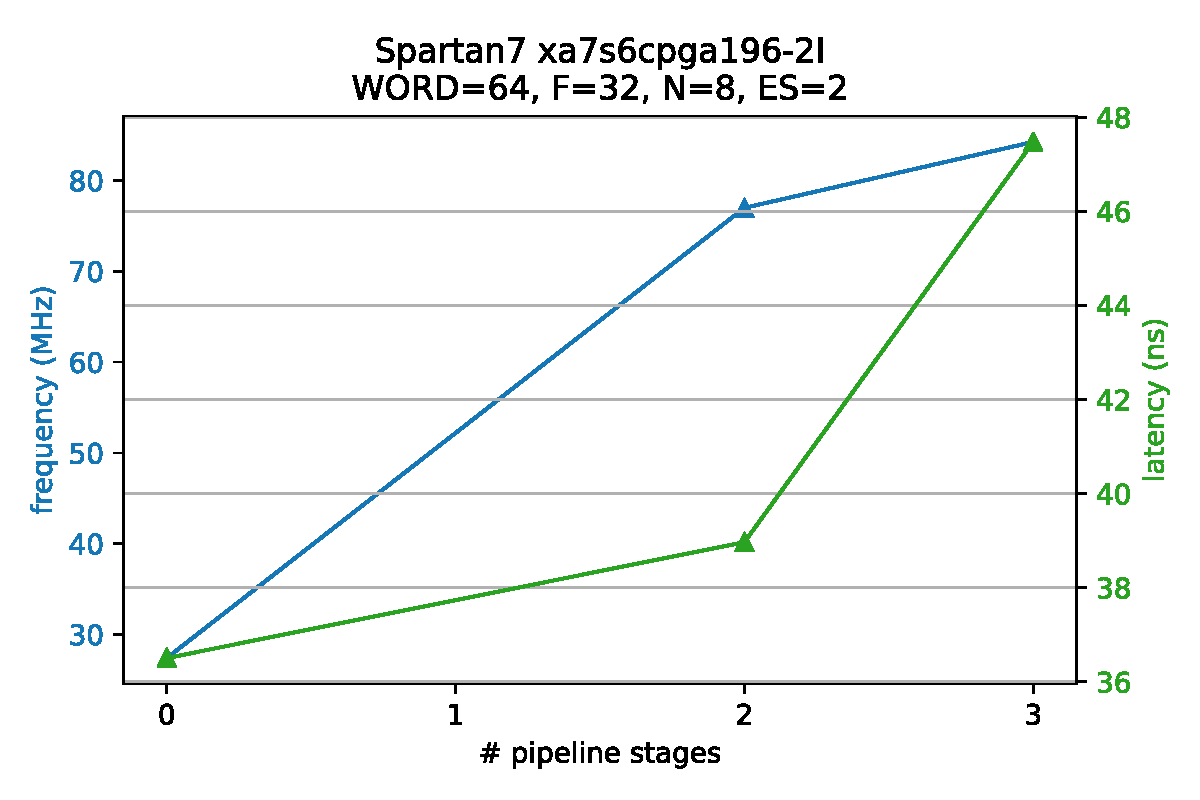
\includegraphics[width=1\textwidth]{figures/Spartan7_xa7s6cpga196-2I_64_32_8_2_freq_lat.pdf}
        \caption{\posit{8}{2} pipeline stages impact on frequency and latency}
        \label{fig:spartan7_stages_vs_freqlatency_64_32_8_2}
\end{figure}
\begin{figure}
    \centering
    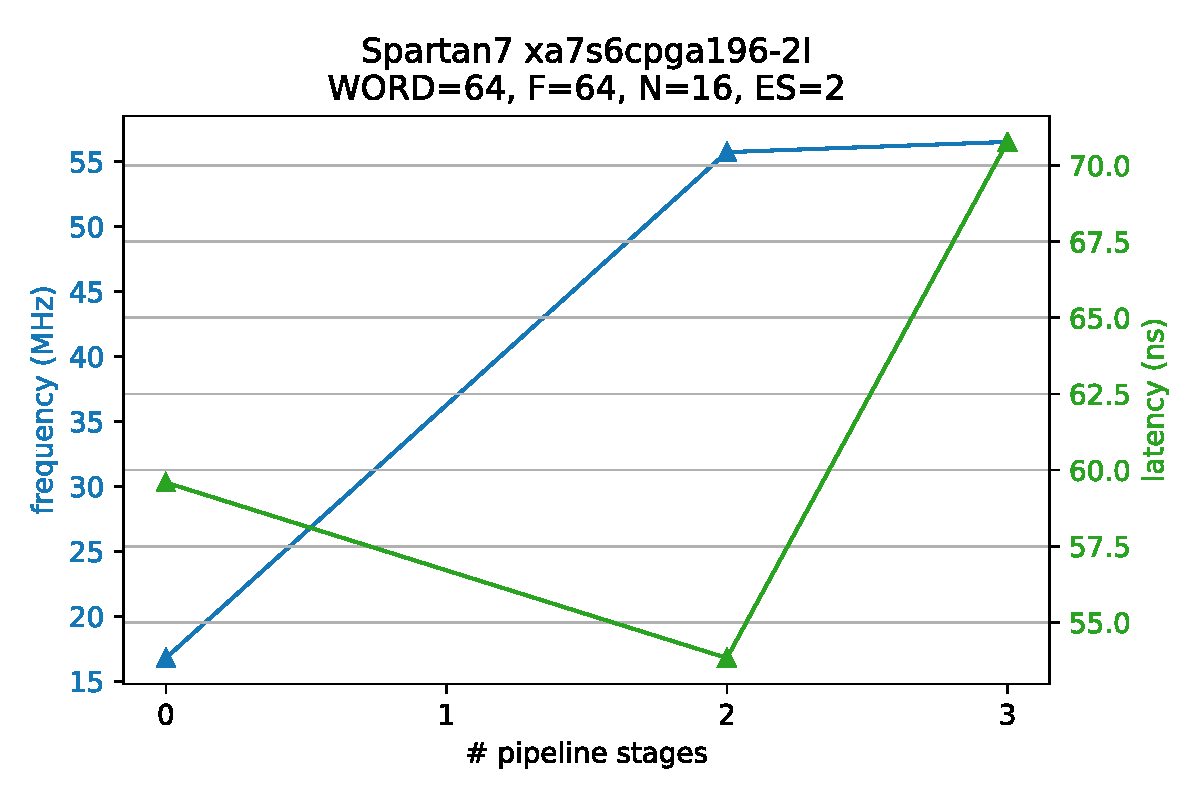
\includegraphics[width=1\textwidth]{figures/Spartan7_xa7s6cpga196-2I_64_64_16_2_freq_lat.pdf}
    \caption{\posit{16}{2} pipeline stages impact on frequency and latency}
    \label{fig:spartan7_stages_vs_freqlatency_64_64_16_2}
\end{figure}




\section{Synthesis and characterization}

\subsection{Power}
Typically, the static power is constant regardless of the circuit's current operating state; indeed, it consists of leakage currents from supply to ground via the transistors.

Meanwhile, the dynamic power is the one consumed by transistors due to the switching activity.

We can model the total power consumption of a circuit as:
\begin{equation}\label{equ:power_cmos_equation}
P_{tot} = \underbrace{V_{CC} \cdot I_{leak}}_{P_{static}} + \underbrace{\alpha \cdot C \cdot V_{CC}^2 \cdot f}_{P_{dynamic}}
\end{equation}

where $V_{CC}$ is the supply voltage, $I_{leak}$ is the total leakage current, $\alpha$ is the activity factor, $C$ is the driven capacitance and $f$ is the operating clock frequency of the circuit.



\subsection{Timing}
Important parameters that affect how much we can drive up the frequency of a design, are the length and latency critical path (i.e. the longest path a signal must travel between two endpoints before the next clock edge).
The worst slack determines the maximum achievable frequency, that is the time we have left before violating register hardware constraints.
If the slack is positive all signals respect the requirements, thus we can achieve a higher frequency, furtherly reducing it. Negative slack means the circuit has timing violations at the given frequency, and we may incur malfunctioning operations.

\subsection{Synthesis}

We generated, tested and validated, several PPU configurations with all their algebraic operations. Then, we used the Xilinx Vivado suite to proceed with the hardware synthesis of our component.


% --------------------------------------------------------


The core logic element of Xilinx FPGAs is the so-called Configurable Logic Block (CLB). A CLB contains logic slices and it is connected to the interconnection matrix via a dedicated switch. Slices are the basic resource used to synthesize designs: in particular, they build Lookup Tables (LUT) and Registers. LUTs can be used to implement complex combinatorial logic while registers are used to implement sequential logic. Additionally, multiplexers are embedded within slices to route internal signals.

The PPU module is intended to be tightly coupled to a more complex system (e.g. a complete processor unit). In order to characterize our unit, we leveraged the out-of-context (OOC) synthesis mode, which simulates the pin connection for inputs and outputs without the need of an external driver.
Synthesizing or implementing a module out of context requires that the tools be run in an ``out-of-context" mode\footnote{\url{https://docs.xilinx.com/r/2021.2-English/ug905-vivado-hierarchical-design/Out-of-Context-Commands}}.

Using the OOC mode has the following implications:
\begin{itemize}
\item external signals are not routed to the I/O pins of the chip. This means that input and output signals do not need to stretch through the entire chip
\item connections are consequently shorter, reducing delays and increasing the space for higher frequencies
\end{itemize}

We run the power, timing and utilization reports on on three different Xilinx FPGA families -- Spartan7, Kintex7, and Virtex UltraScale+ -- using different posit/float datatype formats, as reported in Tables (in Appendix) \ref{table:table_xa7s6cpga196-2I}, \ref{table:table_xc7k325tffg900-2}, \ref{table:table_xcku060-ffva1156-3-e} and \ref{table:table_xcvu23p-fsvj1760-3-e}, respectively.

Tables \ref{table:table_xa7s6cpga196-2I}, \ref{table:table_xc7k325tffg900-2}, \ref{table:table_xcvu23p-fsvj1760-3-e}, \ref{table:table_xcku060-ffva1156-3-e} show  to the following:
\begin{itemize}
    \item the fastest speed can be reached on the Virtex UltraScale+ which -- everything else being equal\footnote{e.g. (WORD, F, N, ES) = (64, 0, 8, 0)} -- can operate at $75 \%$ and $126 \%$ higher clock rate\footnote{highest clock rate defined as the reciprocating of the smallest clock period which, in turn, is defined as the clock period (T) minus the Worst Negative Slack (WNS). WNS is the margin between the current clock period and the smallest clock period the design could operate at, without violating the setup time} than the Kintex7 and Spartan7 respectively. This is a direct consequence of the fabrication technologies of those chips: 16\footnote{Virtex\textregistered UltraScale+\textsuperscript{TM} \url{https://www.xilinx.com/products/silicon-devices/fpga/virtex-ultrascale-plus.html}} vs 28\footnote{Kintex\textregistered-7 \url{https://www.xilinx.com/products/silicon-devices/fpga/kintex-7.html}} vs 28\footnote{Spartan\textregistered-7 \url{https://www.xilinx.com/products/silicon-devices/fpga/spartan-7.html}} nanometers.
    \item longer posit formats run at a slower speed due to the growing (mostly) divider path length,
    %\item larger power is consumed on larger devices -- predominanly \textit{static},
    \item larger power is consumed at higher clock rate -- predominantly \textit{dynamic},
    \item the larger percentage of power consumed on the larger devices is the static component: this comes from keeping the chip powered on, and is not directly related to the actual power drained by the design.
\end{itemize}



\section{Comparison with PACoGEN}

In order to complement and back up the claims stated in section \ref{Approximated_Algorithms}, we choose one of the most common works in the literature related to Posit core generators, to compare our own design against.
PACoGen \cite{PACoGen} is a scientific paper published in mid 2019 where the authors designed one of the first \textbf{p}osit \textbf{a}rithmetic \textbf{co}re \textbf{gen}erators (hence the acronym). The foremost reason why this was chosen as a reference target, is that its HDL implementation was released as open-source\footnote{\url{https://github.com/manish-kj/PACoGen}} under the BSD 3-Clause License.


The source code presents itself as three compartmentalized folders, one for each supported binary operation, i.e. \textit{add}, \textit{mul}, \textit{div}, each of which is implemented in a single HDL description file -- leaving thus little room for code (and resources) reuse.

The promise of PACoGen is to generate cores supporting operations over \textit{any} posit format.

The implementations of the adder and multiplier are as straightforward as they can get, as they can always produce exact results.

 The division, however, has room for compromises and original choices. The way they go around that is the ``approximated algorithm" route: a  LUT storing the $M$ most significant bits of the reciprocate of the fractions followed by $S$ Newton Raphson iterations (Figure \ref{fig:pacoge_divider_architecture}), narrowing down the accuracy at the finest level desired. The number of Newton Raphson iterations is:
    \begin{equation*}\label{equ:regime_k_equation}
        S = \begin{cases}
        0, &\text{ if } N \le 8 \\
        1, &\text{ if } 8 < N \leq 16 \\
        2, &\text{ if } 16 < N \le 32 \\
        \end{cases}
    \end{equation*}
    or, in general, $S = \lceil \log_2(N / 8) \rceil$.

\begin{figure}
    \centering
    \includegraphics[width=0.6\textwidth]{figures/div_pacogen_architecture.pdf}
    \caption{\cite{PACoGen}'s PACoGen divider architecture}
    \label{fig:pacoge_divider_architecture}
\end{figure}


PACoGen does not support out of the box the posit formats $P\langle\_, 0\rangle$, which is unfortunate since, together with $P\langle16, 1\rangle$ and $P\langle32, 2\rangle$, $P\langle8, 0\rangle$ was the standard $8$-bit posit type at the time this work was carried out\footnote{The posit standard was ratified on March 2, 2022 (\url{https://posithub.org/docs/posit_standard-2.pdf}), pinning the exponent size at $2$ for any posit size $N$}.

To work around the limitation of not being able to compare division results between different configurations of posits, we forked the repository and retrofitted all three modules to support the $ES = 0$ posits class.


The result of the comparison (using the setup shown in Figure \ref{fig:comparison_against_pacogogen_dut}), generated by comparing the division module
for all the desired combinations of posit formats is reported in Table \ref{table:comparison_div_against_pacogen_table}, where \textit{LUT\_IN} and \textit{LUT\_OUT} are the sizes of the LUT used to store the precomputed most significant bits of the reciprocate of $\text{mant}_2$, interpreted as \texttt{Fx<1, B>} as wholly described in section \ref{aot_reciprocal_lut_technique}; and \textit{NR} indicates the number of Newton Raphson iterations. These three parameters are hard-coded in the original version of PACoGen.
The ``wrong [\%]" columns report the percentages of results that differ from the ground truth division between two posits: these are tested against our software library (and others, where applicable).
Recall that our divider consists of one Newton Raphson iteration preceded by what has been referred to as \textit{fast reciprocate} (figure \ref{fig:reciprocal_unsigned_workflow}).


These inexactnesses involve, in almost $100 \%$ of the cases, the least significant bit, which is, for the large part, always a fraction bit. This means that these ``errors" are as meaningless as they can get, both for PACoGen and ours.
The benefit provided by our approach in terms of accuracy, up to 16-bits posit, is also crystal clear.


Figure \ref{fig:comparison_against_pacogogen_dut_waveforms} shows waveforms of the comparison between PACoGen and proposed: the last four traces indicate -- when non-zero -- that an inexact posit division happened. The density of the \textit{spikes} gives a qualitative indication of their inexactness. The traces suffixed with \textit{off by 1} indicate that only the least significant bit is off, which is \~ always. These qualitative indicators are quantified in Table \ref{table:comparison_div_against_pacogen_table}.


\begin{figure}
        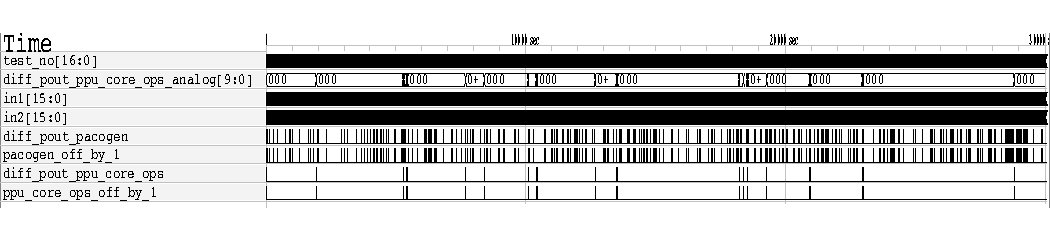
\includegraphics[width=\textwidth]{figures/waveform_div_against_pacogen.pdf}
        \caption{Waveform from the simulation of comparison between PACoGEN and the proposed unit}
        \label{fig:comparison_against_pacogogen_dut_waveforms}
\end{figure}




\begin{table}
\begin{center}
\begin{savenotes}
\begin{tabular}{ccccccccc}
    \toprule
     & & \multicolumn{4}{c}{PACoGen} & & \multicolumn{2}{c}{proposed} \\
    \cmidrule{3-6} \cmidrule{8-9}
    N & ES & LUT IN & LUT OUT & NR & wrong [\%] & & NR & wrong [\%] \\
    \midrule \midrule
    8 & 0 & 8 & 9 & 0 & 4.8 & & 1 & \textbf{1.4} \\
    8 & 1 & 8 & 9 & 0 & 5.4 & & 1 & \textbf{1.2} \\
    8 & 2 & 8 & 9 & 0 & 9.3 & & 1 & \textbf{2.1} \\
    8 & 3 & 8 & 9 & 0 & 13.5 & & 1 & \textbf{4.2} \\
    8 & 4 & 8 & 9 & 0 & 16.4 & & 1 & \textbf{7.5} \\
    \midrule
    16 & 0 & 8 & 9 & 1 & 10.0 & & 1 & \textbf{1.5} \\
    16 & 1 & 8 & 9 & 1 & 10.0 & & 1 & \textbf{0.6} \\
    16 & 2 & 8 & 9 & 1 & 8.8 & & 1 & \textbf{0.5} \\
    16 & 3 & 8 & 9 & 1 & 9.0 & & 1 & \textbf{0.1} \\
    \bottomrule
\end{tabular}
\end{savenotes}
\caption{Percentages of posits $P\langle N,ES\rangle$ inexact division results. \cite{PACoGen}'s PACoGen vs proposed}
\label{table:comparison_div_against_pacogen_table}
\end{center}
\end{table}


\begin{figure}
        \includegraphics[width=\textwidth]{figures/pacogen_vs_me_dut.pdf}
        \caption{Device setup for the comparison between PACoGEN Divider a the proposed one}
        \label{fig:comparison_against_pacogogen_dut}
\end{figure}